\PassOptionsToPackage{dvipsnames,table}{xcolor}
\documentclass[12pt,a4paper,oneside]{report}

%-------------------- Page layout and fonts --------------------------
\usepackage[a4paper,left=1.25in,right=1in,top=1in,bottom=1in,headheight=15pt]{geometry}
% Font: LaTeX default Computer Modern (cmr) throughout --- do not load other font packages
\usepackage{eso-pic}             % page border on front-matter pages
\usepackage{setspace}
\onehalfspacing
\usepackage{microtype}

%-------------------- Packages ---------------------------------------
\usepackage{graphicx}
\usepackage{amsmath,amssymb}
\usepackage{booktabs,tabularx,multirow,longtable,array}
\usepackage{float}
\usepackage[font=small,labelfont=bf]{caption}
\usepackage{enumitem}
\usepackage[dvipsnames,table]{xcolor}
\usepackage{tikz}
\usetikzlibrary{arrows.meta,positioning,shapes.geometric,fit,backgrounds}
\usepackage{pgfplots}
\pgfplotsset{compat=1.17}
\usepackage{algorithm}
\usepackage{algpseudocode}
\usepackage{listings}
\usepackage[most]{tcolorbox}
\usepackage{fancyhdr}
\usepackage{titlesec}
\usepackage{hyperref}
\hypersetup{
    bookmarksopen=true,
    colorlinks=true,
    citecolor=blue,
    linkcolor=blue,
    urlcolor=blue
}

%=====================================================================
%  PROJECT DETAILS --- EDIT THIS BLOCK
%=====================================================================
\newcommand{\ProjectTitle}{LoomTrace: An Agentic Verifier for Geographical Indication Claims on Indian Handloom Products}
% Short title for the page header (shorten if it does not fit on one line)
\newcommand{\HeaderTitle}{LoomTrace: Agentic GI-Claim Verifier for Handloom}
\newcommand{\TeamNo}{10}
\newcommand{\AcademicYear}{2026--27}
\newcommand{\SubmissionDate}{12 November 2026}
% Team members: USN and Name (delete the 4th row in the tables if you have only 3 members)
\newcommand{\USNa}{1BM23CD027}  \newcommand{\NameA}{Sudeeksha}
\newcommand{\USNb}{1BM23CD026}  \newcommand{\NameB}{Khushi Vernekar}
\newcommand{\USNc}{1BM23CD066}  \newcommand{\NameC}{Trishul J}
\newcommand{\USNd}{1BM24CD400}  \newcommand{\NameD}{Geetha R}
% Course lead
\newcommand{\GuideName}{Dr. Kalyan Nagaraj}
\newcommand{\GuideDesig}{Assistant Professor}

%=====================================================================
%  GUIDANCE SWITCH: set to \guidancefalse before final submission
%=====================================================================
\newif\ifguidance
\guidancefalse

%-------------------- Colours and boxes -------------------------------
\definecolor{bmsblue}{RGB}{0,51,102}
\definecolor{guidebg}{RGB}{232,240,252}
\definecolor{dobg}{RGB}{230,245,233}
\definecolor{dontbg}{RGB}{252,232,232}
\definecolor{samplecol}{RGB}{40,55,80}

% "What to write here" box
\newcommand{\guide}[1]{%
  \ifguidance
  \begin{tcolorbox}[enhanced,breakable,colback=guidebg,colframe=bmsblue,
    boxrule=0.6pt,arc=2pt,left=6pt,right=6pt,top=4pt,bottom=4pt,
    fonttitle=\bfseries\small,title={What to write here},
    before upper={\small\setstretch{1.1}}]
  #1
  \end{tcolorbox}
  \fi}

% Do / Don't box (two columns)
\newcommand{\dodont}[2]{%
  \ifguidance
  \begin{tcolorbox}[enhanced,breakable,sidebyside,sidebyside align=top seam,
    colback=dobg,colbacklower=dontbg,colframe=gray!60,boxrule=0.5pt,arc=2pt,
    lefthand ratio=0.5,left=5pt,right=5pt,top=4pt,bottom=4pt,
    fontupper=\small\setstretch{1.05},fontlower=\small\setstretch{1.05}]
  \textbf{\textcolor{ForestGreen}{\checkmark\ Do}}
  \begin{itemize}[leftmargin=12pt,itemsep=1pt,topsep=2pt]#1\end{itemize}
  \tcblower
  \textbf{\textcolor{BrickRed}{$\times$ Don't}}
  \begin{itemize}[leftmargin=12pt,itemsep=1pt,topsep=2pt]#2\end{itemize}
  \end{tcolorbox}
  \fi}

% Page budget note for each chapter
\newcommand{\pagebudget}[1]{%
  \ifguidance\noindent{\small\textcolor{bmsblue}{\textbf{Expected length:} #1 pages}}\par\medskip\fi}

% Sample content marker (sample text is shown in dark slate colour)
\newenvironment{sample}
  {\par\noindent{\footnotesize\bfseries\textcolor{BrickRed}{[SAMPLE --- replace with your own content]}}\par\color{samplecol}}
  {\par\medskip}

%-------------------- Headers and footers ----------------------------
% Main body (Chapter 1 onwards): project title right in header, CSE (Data Science) left and
% page number right in footer, with double rules. Front matter: page border, page number only.
% Double rules (thick + thin, 1.5pt apart), drawn with \hrule so no line spacing is inserted
\newcommand{\DoubleHeadRule}{\vskip 2pt{\color{bmsblue}%
  \hrule width\headwidth height 1.2pt\vskip 1.5pt\hrule width\headwidth height 0.4pt}\vskip -5.1pt}
\newcommand{\DoubleFootRule}{\vskip-\footruleskip\vskip-3.1pt{\color{bmsblue}%
  \hrule width\headwidth height 0.4pt\vskip 1.5pt\hrule width\headwidth height 1.2pt}\vskip\footruleskip}
\fancypagestyle{mainbody}{%
  \fancyhf{}%
  \fancyhead[R]{\small\itshape\HeaderTitle}%
  \fancyfoot[L]{\small CSE (Data Science)}%
  \fancyfoot[R]{\small\thepage}%
  \renewcommand{\headrulewidth}{1pt}\renewcommand{\footrulewidth}{1pt}%
  \renewcommand{\headrule}{\DoubleHeadRule}\renewcommand{\footrule}{\DoubleFootRule}}
\fancypagestyle{frontmatter}{%
  \fancyhf{}\fancyfoot[C]{\small\thepage}%
  \renewcommand{\headrulewidth}{0pt}\renewcommand{\footrulewidth}{0pt}%
  \renewcommand{\headrule}{}\renewcommand{\footrule}{}}
% Double page border (front matter only)
\newcommand{\PageBorder}{%
  \AddToShipoutPictureBG{\AtPageLowerLeft{%
    \setlength{\unitlength}{1pt}%
    \begin{tikzpicture}[remember picture,overlay]
      \draw[bmsblue,line width=1.6pt] ([xshift=1.2cm,yshift=1.2cm]current page.south west)
        rectangle ([xshift=-1.2cm,yshift=-1.2cm]current page.north east);
      \draw[bmsblue,line width=0.5pt] ([xshift=1.35cm,yshift=1.35cm]current page.south west)
        rectangle ([xshift=-1.35cm,yshift=-1.35cm]current page.north east);
    \end{tikzpicture}}}}

%-------------------- Chapter heading style --------------------------
\titleformat{\chapter}[display]
  {\normalfont\bfseries\centering}
  {\Large\textcolor{bmsblue}{CHAPTER \thechapter}}{6pt}{\LARGE\MakeUppercase}
\titlespacing*{\chapter}{0pt}{-10pt}{24pt}
\titleformat{\section}{\normalfont\large\bfseries}{\thesection}{0.6em}{}
\titleformat{\subsection}{\normalfont\normalsize\bfseries}{\thesubsection}{0.6em}{}

%-------------------- Code listing style -----------------------------
\lstset{basicstyle=\ttfamily\footnotesize,breaklines=true,frame=single,
  backgroundcolor=\color{gray!6},numbers=left,numberstyle=\tiny\color{gray},
  keywordstyle=\color{bmsblue}\bfseries,commentstyle=\color{ForestGreen},
  stringstyle=\color{BrickRed},showstringspaces=false,columns=fullflexible,keepspaces=true}

\begin{document}

%=====================================================================
%  TITLE PAGE
%=====================================================================
\pagenumbering{gobble}
\PageBorder
\pagestyle{frontmatter}
\begin{titlepage}
\centering
\setstretch{1.2}
{\large\bfseries B.M.S. COLLEGE OF ENGINEERING}\\[2pt]
{\normalsize (Autonomous Institute, Affiliated to VTU, Belagavi)}\\[2pt]
{\normalsize Bull Temple Road, Basavanagudi, Bengaluru -- 560019}\\[12pt]

\includegraphics[width=3.2cm]{logo.png}\\[14pt]
{\normalsize A Mini-Project Report on}\\[10pt]
{\Large\bfseries\textcolor{bmsblue}{\ProjectTitle}}\\[14pt]
{\normalsize Submitted as the Alternative Assessment Tool (AAT) for the course}\\[2pt]
{\normalsize\bfseries Agentic AI (26CD7PEAAI)}\\[2pt]
{\normalsize of}\\[2pt]
{\normalsize\bfseries Bachelor of Engineering}\\[2pt]
{\normalsize in}\\[2pt]
{\normalsize\bfseries Computer Science and Engineering (Data Science)}\\[14pt]
{\normalsize Submitted by (Team No.\ \TeamNo)}\\[6pt]
\renewcommand{\arraystretch}{1.3}
\begin{tabular}{l@{\hspace{1.5cm}}l}
\textbf{\USNa} & \textbf{\NameA} \\
\textbf{\USNb} & \textbf{\NameB} \\
\textbf{\USNc} & \textbf{\NameC} \\
\textbf{\USNd} & \textbf{\NameD} \\
\end{tabular}\\[16pt]
{\normalsize Course Lead}\\[4pt]
{\large\bfseries \GuideName}\\[2pt]
{\normalsize \GuideDesig, Department of CSE (Data Science)}\\[2pt]
{\normalsize B.M.S. College of Engineering, Bengaluru}\\[16pt]
\vfill
{\normalsize\bfseries Department of Computer Science and Engineering (Data Science)}\\[2pt]
{\normalsize B.M.S. College of Engineering, Bengaluru}\\[2pt]
{\normalsize Academic Year \AcademicYear}
\end{titlepage}

%=====================================================================
%  FRONT MATTER
%=====================================================================
\pagenumbering{roman}
\setcounter{page}{2}

%-------------------- Certificate ------------------------------------
\chapter*{Certificate}
\addcontentsline{toc}{chapter}{Certificate}
\thispagestyle{frontmatter}
\begin{center}

\includegraphics[width=2.2cm]{logo.png}\\[6pt]
{\bfseries B.M.S. College of Engineering, Bengaluru}\\
Department of Computer Science and Engineering (Data Science)
\end{center}
\vspace{10pt}
This is to certify that the mini-project entitled \textbf{``\ProjectTitle''} has been carried out by
\NameA\ (\USNa), \NameB\ (\USNb), \NameC\ (\USNc) and \NameD\ (\USNd), bona fide students of
B.M.S. College of Engineering, Bengaluru, as the Alternative Assessment Tool (AAT) for the evaluation
of the course \textbf{Agentic AI (26CD7PEAAI)}, Semester VII, Bachelor of Engineering in Computer
Science and Engineering (Data Science), during the academic year \AcademicYear. The work has been
evaluated through the four project reviews prescribed for the course, and this report satisfies the
requirements of the AAT component of the said course.

\vspace{70pt}
\noindent\hfill
\begin{minipage}[t]{0.62\textwidth}\raggedleft
\rule{6cm}{0.4pt}\\
\textbf{\GuideName}\\
Course Lead, Agentic AI (26CD7PEAAI)\\
\GuideDesig, Dept. of CSE (Data Science)\\
B.M.S. College of Engineering, Bengaluru\\[10pt]
Date: \rule{3.5cm}{0.4pt}
\end{minipage}

%-------------------- Abstract ---------------------------------------
\chapter*{Abstract}
\addcontentsline{toc}{chapter}{Abstract}
\thispagestyle{frontmatter}
Handloom products in India are frequently sold with claims of a Geographical Indication (GI) tag,
such as Kancheepuram Silk or Pochampalli Ikat, but a buyer or marketplace has no quick way to check
whether such a claim is backed by official records. The evidence needed is spread across the GI
registry, the GI application documents, the national handloom census and producer records, and a
single prompt to a language model can neither consult these sources nor guarantee that its answer is
grounded in them. This report presents LoomTrace, an agent that checks a GI claim on a handloom product
and returns an advisory, cited verdict: Supported, Conflicting evidence, or Insufficient evidence, the
last of which is routed to a human reviewer. LoomTrace is implemented as a LangGraph state graph of six
nodes (extraction, planning, a retriever agent, a verifier agent, an evidence grader and a guardrail)
with a bounded re-planning loop, seven typed tools, keyword-based retrieval over official GI text,
per-node checkpoints in an SQLite database, and a web interface with a review queue. Reference data
cover fifteen GI-registered handloom products and the state-wise weaver counts of the Fourth All India
Handloom Census 2019--20; individual weaver and production records are simulated. On a labelled set of
45 cases the agent reached 100\% verdict accuracy and correctly routed all 15 unclear cases to human
review, while a single-lookup baseline reached 33.3\% and never abstained. Disabling the re-planning
loop reduced accuracy to 80.0\%, at a mean saving of 3.1 milliseconds per case. The main limitation is
that the test set was constructed by the team from simulated producer records, so these results
demonstrate correct behaviour on controlled cases rather than accuracy on real marketplace listings.

\medskip
\noindent\textbf{Keywords:} agentic AI, geographical indications, handloom, retrieval-augmented
generation, human-in-the-loop, LangGraph.

%-------------------- Lists ------------------------------------------
\tableofcontents
\listoffigures
\addcontentsline{toc}{chapter}{List of Figures}
\listoftables
\addcontentsline{toc}{chapter}{List of Tables}

\chapter*{List of Abbreviations}
\addcontentsline{toc}{chapter}{List of Abbreviations}
\thispagestyle{frontmatter}
\begin{tabular}{@{}p{2.8cm}l@{}}
API & Application Programming Interface \\
BM25 & Best Matching 25 (Okapi ranking function) \\
GI & Geographical Indication \\
HITL & Human-in-the-Loop \\
IP & Intellectual Property \\
JSON & JavaScript Object Notation \\
LLM & Large Language Model \\
OCR & Optical Character Recognition \\
PIB & Press Information Bureau \\
RAG & Retrieval-Augmented Generation \\
ReAct & Reasoning and Acting \\
SLM & Small Language Model \\
TRIFED & Tribal Co-operative Marketing Development Federation of India \\
TRIPS & Trade-Related Aspects of Intellectual Property Rights \\
UI & User Interface \\
\end{tabular}

%=====================================================================
%  MAIN BODY
%=====================================================================
\clearpage
\ClearShipoutPictureBG
\pagestyle{mainbody}
\fancypagestyle{plain}{\pagestyle{mainbody}}
\pagenumbering{arabic}

%---------------------------------------------------------------------
\chapter{Introduction}
%---------------------------------------------------------------------

This chapter introduces the handloom sector and the problem of verifying Geographical Indication (GI)
claims on handloom products. It states the decision that the proposed agent supports, explains why an
agentic design is needed rather than a script or a single language-model prompt, and sets out the
objectives and scope of the project.

\section{Background}

A Geographical Indication is a sign used on goods that have a specific geographical origin and that
possess qualities, a reputation or characteristics essentially attributable to that origin. The
Agreement on Trade-Related Aspects of Intellectual Property Rights (TRIPS) requires member countries
to provide legal means to prevent the use of a geographical indication on goods that do not originate
in the indicated area~\cite{trips}. In India this obligation is implemented by the Geographical
Indications of Goods (Registration and Protection) Act, 1999, under which a GI is registered by an
association of producers, and individual producers may in turn be registered as authorised
users~\cite{giact1999}. Registrations are maintained by the Geographical Indications Registry of the
Office of the Controller General of Patents, Designs and Trade Marks, commonly referred to as IP
India~\cite{ipindia}.

Handloom textiles form one of the largest groups of registered Indian GIs. Products such as
Kancheepuram Silk from Tamil Nadu, Pochampalli Ikat from Telangana, Banaras Brocades and Sarees from
Uttar Pradesh, Sambalpuri Bandha from Odisha and Chanderi Sarees from Madhya Pradesh are each tied to
named districts, weaving communities, materials and techniques~\cite{ipindia,pibgi}. The sector is
large and dispersed: according to the Fourth All India Handloom Census 2019--20, India has
26,73,891 handloom weavers and 8,48,621 allied workers, with the largest weaver populations in
Assam (11,07,428), West Bengal (3,66,656) and Manipur (2,12,481)~\cite{pibcensus}. For the three
products on which this project was first scoped, the census records 1,97,818 handloom weavers in
Tamil Nadu, 25,930 in Telangana and 1,30,778 in Uttar Pradesh~\cite{pibcensus}.

Because a GI signals both origin and traditional method, a GI claim adds commercial value to a product,
and it is used prominently in product descriptions, labels and online listings. The Ministry of
Textiles operates certification schemes such as the Handloom Mark and the India Handloom Brand to help
buyers identify genuine handloom goods~\cite{handloommark}. However, a buyer or a marketplace operator
who sees the claim ``GI-tagged Kanjivaram silk saree'' on a listing still has to establish several
separate facts before trusting it: that the product name corresponds to a registered GI, that the
stated place of manufacture lies within the registered geographical area, that the materials are
consistent with the registered description, and that the weaver and production batch can be traced to
the relevant weaving cluster.

\section{Problem Statement}

A buyer, marketplace moderator or cooperative officer who receives a handloom product with a GI-tag
claim has no single place to check whether the claim is supported. The necessary evidence is spread
across the GI registration list, the statement of case in each GI application, the national handloom
census and producer-level weaver and batch records, and the product label itself may use a local
name (``Kanjivaram'' instead of ``Kancheepuram Silk''), omit identifiers, or contain details that
contradict the registration. Checking these sources manually is slow and inconsistent, and an
unsupported claim may be accepted while a genuine product with incomplete paperwork may be wrongly
rejected. \textbf{The decision supported by this project is: is this handloom product's GI-tag claim
supported by the available official evidence, contradicted by it, or not decidable without a human
reviewer?}

\section{Motivation and Why Agentic AI}

Three simpler alternatives were considered before an agentic design was adopted.

\paragraph{A fixed rule script.} A script could compare a structured form against a lookup table.
However, product labels are free text, products are referred to by local names and spellings
(``Pochampally'', ``Ikkat'', ``Banarasi''), and the set of checks that is meaningful depends on which
fields are present: a label without a batch number cannot be checked against provenance records, and
a product that is registered for a whole state (for example, Muga Silk of Assam) must be checked
differently from one registered for specific districts. A fixed pipeline either fails on such inputs or
silently skips checks.

\paragraph{A single language-model prompt.} A large language model (LLM) asked ``is this saree
authentic?'' will answer from its training data. It cannot consult the current registry, it cannot
query producer records, and its output cannot be traced to a source. Language models are known to
produce fluent but unsupported statements~\cite{ji2023hallucination}, and smaller models are
particularly weak when relevant facts are buried in long contexts~\cite{liu2024lost}. For a decision
that affects a producer's reputation, an answer without citations is not acceptable.

\paragraph{Plain retrieval followed by one answer.} A single document lookup followed by one decision
improves grounding, but it cannot notice that its first search failed (for example, because the label
used an alias), and it has no mechanism to stop and ask a human when evidence is missing. Chapter~7
shows that such a baseline marks every case in the test set as ``Supported''.

The problem therefore requires several capabilities that together motivate an agentic design. It
requires \emph{tool use}, because facts must come from registry, census and producer records rather
than from model memory~\cite{schick2023toolformer}. It requires \emph{retrieval over official
documents}, so that every verdict can cite the registered description~\cite{lewis2020rag}. It requires
\emph{planning and re-planning}, because the checks needed differ by claim and a weak first search must
be detected and repeated with a better query~\cite{yan2024crag}. It requires \emph{evidence grading
(reflection)} before a verdict is issued, so that the agent does not guess when evidence is incomplete.
Finally, it requires \emph{human-in-the-loop (HITL) escalation}, because abstaining and referring a case
to a reviewer is safer than wrongly certifying or wrongly rejecting a product.

\section{Objectives}

The objectives of the project are as follows.

\begin{enumerate}[itemsep=2pt]
\item To design an agent, implemented as a state graph, that verifies a handloom GI claim against
official GI and census data and producer records, and returns one of three advisory verdicts with
citations.
\item To implement seven typed tools and retrieval over official GI text, with a bounded re-planning
loop (at most three iterations) that refines the search when the first attempt is weak.
\item To implement a guardrail and a human review workflow so that every case without sufficient,
cited evidence is routed to a reviewer, whose decision is recorded and visible to the requester.
\item To record a step-level trace and a persistent checkpoint for every node of every run.
\item To evaluate the agent on a labelled set of 45 cases against a single-lookup baseline, with
targets of at least 80\% verdict accuracy and at least 90\% correct abstention.
\item To measure, through a controlled A/B experiment, the effect of the re-planning loop on accuracy,
latency and tool usage.
\end{enumerate}

\section{Scope of the Project}

\paragraph{Included.} The system verifies GI-tag claims for fifteen registered handloom GIs: the three
products named in the project's design document (Kancheepuram Silk, Pochampalli Ikat, and Banaras
Brocades and Sarees) and twelve further handloom GIs whose geographical area and materials are stated
in a Government of India GI catalogue~\cite{pibgi}. Input is a product label or seller claim
containing some or all of the following fields: product name, region, state, material, weaver
identifier and batch identifier. Output is an advisory verdict with the list of checks performed and
the sources cited. The system includes a web interface for requesters, a reviewer dashboard, and an
offline evaluation harness.

\paragraph{Excluded.} The system does not issue legal certification and does not replace the GI
Registry or the authorised-user process under the GI Act~\cite{giact1999}. It does not physically
inspect textiles. It does not access live government portals at run time; reference data are stored
locally. Individual weaver and batch records are not publicly available, and the records used are
simulated, as stated in Section~3.4. Products outside the fifteen GIs are reported as ``not covered''
and may be sent to a reviewer, but they are not verified automatically. Label images are supported
only when the optional optical character recognition (OCR) package is installed, and this path was not
part of the evaluation.

\section{Organisation of the Report}

Chapter~2 reviews how GI claims are verified in practice and the technical literature on tool use,
retrieval, planning, reflection and evaluation. Chapter~3 states the stakeholders, requirements and
data sources. Chapter~4 presents the architecture of LoomTrace, its components, the agentic patterns
chosen and the control and data flow. Chapter~5 maps the system to the agentic concepts of the course
with evidence from real runs. Chapter~6 describes the implementation, including the technology stack,
the agent loop, the tools, the guardrails and the user interface. Chapter~7 describes tracing and
reports the evaluation against a baseline, and Chapter~8 reports the A/B experiment on the re-planning
loop. Chapter~9 discusses limitations, failure modes and ethical considerations, and Chapter~10
concludes with future work.

%---------------------------------------------------------------------
\chapter{Literature Survey and Existing Practice}
%---------------------------------------------------------------------

This chapter first describes how GI claims on handloom products are established and checked in
practice, and then reviews the technical literature on the agentic techniques used in LoomTrace. It
ends with a comparative summary and a statement of the gap that the project addresses.

\section{Existing Practice in the Sector}

\subsection{Legal basis of a GI claim}

Under the Geographical Indications of Goods (Registration and Protection) Act, 1999, a GI is
registered for a class of goods and a defined geographical area on the application of an association
of persons or producers. The application contains a \emph{statement of case} that describes the
product, the geographical area, the method of production, the materials and the link between the
product and its origin~\cite{giact1999}. After registration, producers within the area may apply to
be registered as \emph{authorised users}, and only the registered proprietor and authorised users have
the right to use the indication. The registry and its records are maintained by IP India~\cite{ipindia}.
The international basis for this protection is Section~3 of the TRIPS Agreement, which defines
geographical indications and obliges members to prevent misleading use of them~\cite{trips}.

\subsection{How a claim is checked today}

In practice, the verification of a GI claim at the point of sale is manual and fragmented. A buyer in
a shop or on an online marketplace sees a product description or label. To check the claim, the buyer
or a marketplace moderator must find the corresponding GI registration and its application number,
read the statement of case to learn the registered area and materials, and compare these with the
place and materials stated by the seller. Where producer details are provided, they must be checked
against cooperative or weaver records, which are not published centrally. The Ministry of Textiles
supports buyer confidence through separate labelling schemes, notably the Handloom Mark, which
certifies that a product is handwoven, and the India Handloom Brand, which certifies quality and
process standards~\cite{handloommark}. These labels are useful signals, but they do not certify that a
product falls within a particular GI, and they are not linked to the GI registry in a way that a buyer
can query.

Government publications provide some of the reference data needed for verification. The TRIFED GI
catalogue published through the Press Information Bureau (PIB) lists registered GI products marketed
by Tribes India together with short descriptions of their place of production and
materials~\cite{pibgi}. The state-wise results of the Fourth All India Handloom Census 2019--20,
published as a PIB annexure, give the number of handloom weavers and allied workers in each state and
union territory~\cite{pibcensus}. These sources are authoritative but are distributed as separate PDF
documents with different structures, and none of them is designed to answer the question ``is this
particular claim supported?''.

\subsection{Where current practice fails}

Three weaknesses of current practice motivate this project. First, the evidence is spread across
several documents that must be read together, so a complete check is slow and is rarely performed
for an individual purchase. Second, product names on labels and listings frequently differ from the
registered names, which makes simple string search unreliable. Third, when information is missing,
there is no defined route for escalation: the checker must either accept or reject the claim without
evidence, or abandon the check. A system that collects the evidence, explains which checks passed and
failed, and routes undecidable cases to a person addresses all three weaknesses.

\section{Related Technical Work}

The technical literature relevant to LoomTrace is organised below into four themes: reasoning and
acting with tools; retrieval-augmented generation; planning, reflection and multi-agent
collaboration; and the evaluation of systems built on language models.

\subsection{Reasoning and Acting with Tools}

Yao \emph{et al.}~\cite{yao2023react} proposed ReAct, in which a language model interleaves
free-text reasoning steps with actions such as search queries, so that it can gather information
before answering. Schick \emph{et al.}~\cite{schick2023toolformer} showed that a language model can
learn to decide when to call external tools such as calculators and search engines, and how to use
their results. Both works establish that grounding a model's output in tool results reduces reliance
on memorised knowledge. LoomTrace adopts the tool-use principle, since every fact used in a verdict is
returned by a typed tool with a source identifier. It does not, however, adopt free-form interleaving
of thought and action: the sequence of nodes is fixed by an explicit graph, so that every run can be
traced, bounded and checkpointed. This trade-off favours auditability over flexibility, which suits a
verification task whose steps are known in advance.

\subsection{Retrieval-Augmented Generation}

Lewis \emph{et al.}~\cite{lewis2020rag} introduced retrieval-augmented generation (RAG), which
conditions a generator on passages retrieved from an external corpus, and showed gains on
knowledge-intensive tasks. Gao \emph{et al.}~\cite{gao2023ragsurvey} survey later developments and
distinguish naive RAG, which retrieves once, from advanced and modular variants that rewrite queries,
re-rank results and retrieve iteratively. Two adaptive variants are particularly relevant. Self-RAG,
proposed by Asai \emph{et al.}~\cite{asai2024selfrag}, trains a model to decide when to retrieve and to
critique its own output with reflection tokens. Corrective RAG, proposed by Yan
\emph{et al.}~\cite{yan2024crag}, adds a lightweight evaluator that grades retrieved documents and
triggers corrective actions, such as a new search, when retrieval is weak. LoomTrace follows the
corrective pattern: its grader detects when the registry lookup or the document search did not
resolve the product, and the planner then re-queries with the canonical product name and a filter on
that product. For ranking, LoomTrace uses the BM25 function from the probabilistic relevance
framework of Robertson and Zaragoza~\cite{robertson2009bm25}, which is fast, transparent and effective
on short, keyword-rich official passages.

\subsection{Planning, Reflection and Multi-Agent Collaboration}

Wang \emph{et al.}~\cite{wang2023plansolve} proposed plan-and-solve prompting, in which a model first
devises a plan that divides a task into subtasks and then executes it, which reduces missed steps
compared with direct reasoning. Shinn \emph{et al.}~\cite{shinn2023reflexion} proposed Reflexion, in
which an agent evaluates its own attempt and uses verbal feedback to improve the next attempt. Wu
\emph{et al.}~\cite{wu2023autogen} presented AutoGen, a framework in which several specialised agents
converse to complete a task. A survey by Wang \emph{et al.}~\cite{wang2024survey} organises agents built
on language models by their profile, memory, planning and action modules. LoomTrace draws on each of
these ideas in a constrained form. A planner decides which checks a claim requires; a grader evaluates
the evidence before any verdict is produced and can send control back to the planner; and the
gathering of evidence and the judging of evidence are assigned to two separate nodes, a retriever agent
and a verifier agent, with the graph acting as the supervisor that routes between them.

\subsection{Evaluation of LLM-Based Systems}

Zheng \emph{et al.}~\cite{zheng2023judge} studied the use of strong language models as judges of other
models' outputs and reported high agreement with human preferences, while documenting position,
verbosity and self-enhancement biases. Ji \emph{et al.}~\cite{ji2023hallucination} survey hallucination
in natural language generation and emphasise that fluency is not evidence of faithfulness. Liu
\emph{et al.}~\cite{liu2024lost} show that models use information at the beginning and end of long
contexts better than information in the middle. For LoomTrace, these findings have two consequences.
First, because each verdict is one of three discrete labels and each check has a deterministic expected
outcome, the system is evaluated with exact-match metrics against hand-assigned labels rather than with
a model judge. Second, the design keeps every model call narrow and short and assigns the factual checks
to deterministic rules, which is consistent with the known weaknesses of small models on long inputs.

\section{Comparative Summary}

Table~\ref{tab:lit} compares the most relevant approaches with LoomTrace on four properties: whether
the approach calls external tools, whether retrieval is adaptive (graded and repeated when weak),
whether it includes a human escalation path, and whether every decision is accompanied by citations to
sources.

\begin{table}[H]
\centering
\caption{Comparison of related approaches with the proposed system}
\label{tab:lit}
\small
\begin{tabularx}{\linewidth}{@{}>{\raggedright\arraybackslash}p{3.2cm} >{\raggedright\arraybackslash}X c c c c@{}}
\toprule
\textbf{Work} & \textbf{Key idea} & \textbf{Tools} & \textbf{Adapt. RAG} & \textbf{HITL} & \textbf{Cited} \\ \midrule
ReAct~\cite{yao2023react} & Interleaved reasoning and acting & \checkmark & -- & -- & -- \\
Toolformer~\cite{schick2023toolformer} & Self-taught tool calling & \checkmark & -- & -- & -- \\
RAG~\cite{lewis2020rag} & Retrieval-conditioned generation & -- & -- & -- & \checkmark \\
Self-RAG~\cite{asai2024selfrag} & Learned retrieval and self-critique & -- & \checkmark & -- & \checkmark \\
CRAG~\cite{yan2024crag} & Retrieval grading and correction & -- & \checkmark & -- & \checkmark \\
Reflexion~\cite{shinn2023reflexion} & Verbal self-feedback across attempts & \checkmark & -- & -- & -- \\
Manual GI check~\cite{giact1999,ipindia} & Person reads registry and records & -- & -- & \checkmark & \checkmark \\
\textbf{LoomTrace (ours)} & Graph agent with graded re-query and review queue & \checkmark & \checkmark & \checkmark & \checkmark \\
\bottomrule
\end{tabularx}
\end{table}

\section{Research Gap}

As Table~\ref{tab:lit} shows, the general agent techniques reviewed provide tool use, adaptive
retrieval or self-critique individually, but they are not applied to GI verification, and none of them
defines an escalation path to a human reviewer. Manual verification provides human judgement and
citations but does not scale and has no structured way of handling missing information. No reviewed
approach combines retrieval over official GI text, structured checks against registry, census and
producer records, a bounded re-planning loop, and a human review workflow in a single traceable
system for handloom GI claims; LoomTrace is designed to address this gap.

%---------------------------------------------------------------------
\chapter{Requirements and System Analysis}
%---------------------------------------------------------------------

This chapter translates the problem stated in Chapter~1 into concrete requirements. Each functional
requirement is numbered so that it can be traced to the design in Chapter~4 and tested in Chapter~7,
and each non-functional requirement is given a numerical bound.

\section{Stakeholders and Users}

Four groups interact with or are affected by LoomTrace.

\begin{itemize}[itemsep=2pt]
\item \textbf{Requesters (primary users).} Buyers of handloom products, marketplace moderators who
review seller listings, and retail staff who receive stock described as GI-tagged. They need a quick,
understandable answer with the reasons and sources behind it, and a reference number with which to
follow up.
\item \textbf{Reviewers.} Staff of a weavers' cooperative society, a handloom development office or a
marketplace trust-and-safety team who resolve cases that the agent cannot decide. They need the
extracted claim, the reason for escalation and a way to record a decision with a note.
\item \textbf{Weavers and GI proprietors (affected parties).} Producers within the registered area
benefit when false claims are detected, but are harmed if a genuine product is wrongly marked as
conflicting. Their interest is the main reason that the system abstains rather than guesses.
\item \textbf{Course evaluators and developers.} They need step-level traces, reproducible evaluation
scripts and clear documentation of what is real and what is simulated.
\end{itemize}

\section{Functional Requirements}

\begin{description}[leftmargin=1.6cm,style=nextline,itemsep=2pt]
\item[FR1] The system shall accept a product claim as free label text containing any subset of the
fields product, region, state, material, weaver identifier and batch identifier, and optionally a
label image.
\item[FR2] The system shall extract these fields into a typed structure and resolve local product
names and aliases to the registered GI name.
\item[FR3] The system shall decide which checks are applicable to the claim and run them using tools
over the GI registry, GI document text, census data, weaver records and batch records.
\item[FR4] The system shall output exactly one of three verdicts, \emph{Supported}, \emph{Conflicting
evidence} or \emph{Insufficient evidence}, together with the result of every check and the source
identifiers that support it.
\item[FR5] The system shall re-plan and retrieve again when the product cannot be resolved or the
retrieved GI text is weak, for at most three iterations in total.
\item[FR6] The system shall send every \emph{Insufficient evidence} verdict, and any verdict without a
citation or below a confidence threshold, to a human review queue, and shall allow a requester to ask
for review of any verdict.
\item[FR7] The system shall allow a reviewer to record a final decision with a note, and shall allow
the requester to see that decision using the case reference.
\item[FR8] The system shall store the full case state after every node, and keep a history of all
cases and decisions.
\item[FR9] The system shall report claims for products outside the covered GIs as ``not covered''
rather than as conflicting.
\end{description}

\section{Non-Functional Requirements}

\begin{description}[leftmargin=1.6cm,style=nextline,itemsep=2pt]
\item[NFR1] \textbf{Latency.} A verdict shall be returned in under 15 seconds per case, the target set
in the project's design document.
\item[NFR2] \textbf{Bounded cost.} The agent shall execute at most three planning iterations per case,
and therefore at most fifteen tool calls; in rule mode it shall make no paid API calls.
\item[NFR3] \textbf{Traceability.} Every node execution shall be recorded with its inputs and outputs,
and every verdict shall list its source identifiers.
\item[NFR4] \textbf{Safety.} No \emph{Supported} or \emph{Conflicting} verdict shall be issued without at
least one citation and a grade of at least 0.6; otherwise the agent shall abstain.
\item[NFR5] \textbf{Quality.} Verdict accuracy on the labelled test set shall be at least 80\%, and at
least 90\% of cases labelled \emph{Insufficient evidence} shall be routed to human review.
\item[NFR6] \textbf{Reproducibility.} All reported numbers shall be reproducible by running the
scripts in the repository on a laptop without internet access.
\end{description}

\section{Data Sources}

Table~\ref{tab:data} lists the data sources used. Two of them are official Government of India
publications, one is the IP India registration information recorded in the project's design document,
and the producer-level records are simulated because individual weaver and batch data are not
published.

\begin{table}[H]
\centering
\caption{Data sources used in LoomTrace}
\label{tab:data}
\small
\begin{tabularx}{\linewidth}{@{}>{\raggedright\arraybackslash}p{3.0cm} >{\raggedright\arraybackslash}X >{\raggedright\arraybackslash}p{2.1cm} >{\raggedright\arraybackslash}p{3.1cm}@{}}
\toprule
\textbf{Source} & \textbf{Description and use} & \textbf{Size} & \textbf{Origin} \\ \midrule
GI registry entries (3 products) & GI application number, state, districts and materials for Kancheepuram Silk (GI~15), Pochampalli Ikat (GI~4) and Banaras Brocades and Sarees (GI~99); registry checks & 3 records & IP India registration list~\cite{ipindia}, as recorded in the design document \\
GI catalogue (12 products) & Place of production, materials and description of 12 further handloom GIs; registry checks and retrieval corpus & 12 records, 12 passages & PIB / TRIFED, Nov.~2021~\cite{pibgi} \\
GI description passages (3 products) & Short summaries of the registered area, method and materials; retrieval corpus & 9 passages & Written by the team from the GI descriptions; page numbers indicative \\
Handloom census & Handloom weavers and allied workers per state/UT; plausibility check & 31 rows & PIB annexure, release ID 2202869~\cite{pibcensus} \\
Weaver registry & Weaver identifier, name, cluster, district, looms & 180 records & \textbf{Simulated} (seeded generator) \\
Production batches & Batch identifier, weaver, loom, yarn, start and finish dates & 360 records & \textbf{Simulated} (seeded generator) \\
Golden test set & Labelled claims, 3 products $\times$ 3 verdicts $\times$ 5 & 45 cases & Constructed by the team \\
Demonstration tests & Hand-written claims covering 9 products & 15 cases & Constructed by the team \\
\bottomrule
\end{tabularx}
\end{table}

The government data were obtained by downloading the two PIB PDF documents and extracting their text.
The census table was transcribed in full, including all 31 states and union territories. From the GI
catalogue, only handloom textile entries whose place of production is stated in the document were
used; two handloom entries, Khandua Saree and Karvath Kati Sarees, were excluded because the catalogue
does not name their area of production. The catalogue does not print GI application numbers, so for
these twelve products the system reports ``Registered GI'' without a number rather than supplying a
number from an unverified source.

The weaver and batch records are generated by a seeded pseudo-random generator (seed 42), so the same
records are produced on every run. For each product, 12 weavers are assigned in rotation to the
districts of that product's GI area, and each weaver is given two batches whose yarn is drawn from the
product's registered materials. These records are labelled as simulated in the source code, in the
tool outputs (``SIMULATED record'') and in the user interface.

\section{Hardware and Software Requirements}

Development and all evaluation runs used an Apple MacBook with an M2 processor and 8~GB of memory,
running macOS 15.6. The software is written in Python~3.13 and uses LangGraph for orchestration,
Pydantic for typed tool schemas, SQLite for persistence, Streamlit for the interface and pandas for
tabular display. The optional language-model path uses the Groq API with the Llama~3.1~8B Instant
model, and the optional OCR path uses EasyOCR. Exact versions are given in Table~\ref{tab:stack} and
Appendix~\ref{app:run}. No graphics processor is required.

\section{Feasibility}

\paragraph{Technical feasibility.} All checks reduce to lookups and comparisons over small tables and a
corpus of 21 passages, so they can be executed in milliseconds on a laptop. The only components that
require external services, the language model and OCR, are optional and are isolated behind tool
interfaces with deterministic fall-backs.

\paragraph{Cost.} All results in this report were produced in rule mode, without an API key, and
therefore made zero language-model calls and incurred no cost. In the optional model mode, the design
limits model usage to two short calls per case (field extraction and verdict explanation); the model
selected is available on the free tier of the Groq service~\cite{groq}.

\paragraph{Time and scope control.} The scope was limited to verification against stored reference data;
live access to government portals was avoided because the IP India application-detail pages returned
errors during data collection and because the evaluation must be reproducible offline. The project
was initially scoped to three products, as specified in the design document, and was extended to
fifteen products once the official GI catalogue had been obtained.

%---------------------------------------------------------------------
\chapter{Agent Design and Architecture}
%---------------------------------------------------------------------

This chapter presents the architecture of LoomTrace, describes each component shown in the
architecture diagram, justifies the agentic patterns that were selected against the alternatives that
were rejected, and describes the control flow, the shared state and the flow of data through the
system for one concrete input.

\section{System Architecture}

Figure~\ref{fig:arch} shows the architecture of LoomTrace. A product claim enters at the top left and
passes through six nodes of a state graph: \emph{Extract}, \emph{Planner}, the \emph{Retriever agent},
the \emph{Verifier agent}, the \emph{Grader} and the \emph{Guardrail}. The retriever agent calls typed
tools that read four data stores. The grader decides whether the evidence is sufficient; if it is not,
control returns to the planner, at most three times in total. The guardrail issues the verdict with its
citations, or escalates the case to a review queue, from which a human reviewer records the final
decision. All nodes read and write a single shared state object, \texttt{CaseState}, which is saved to
an SQLite database after every node.

\begin{figure}[H]
\centering
\resizebox{\linewidth}{!}{%
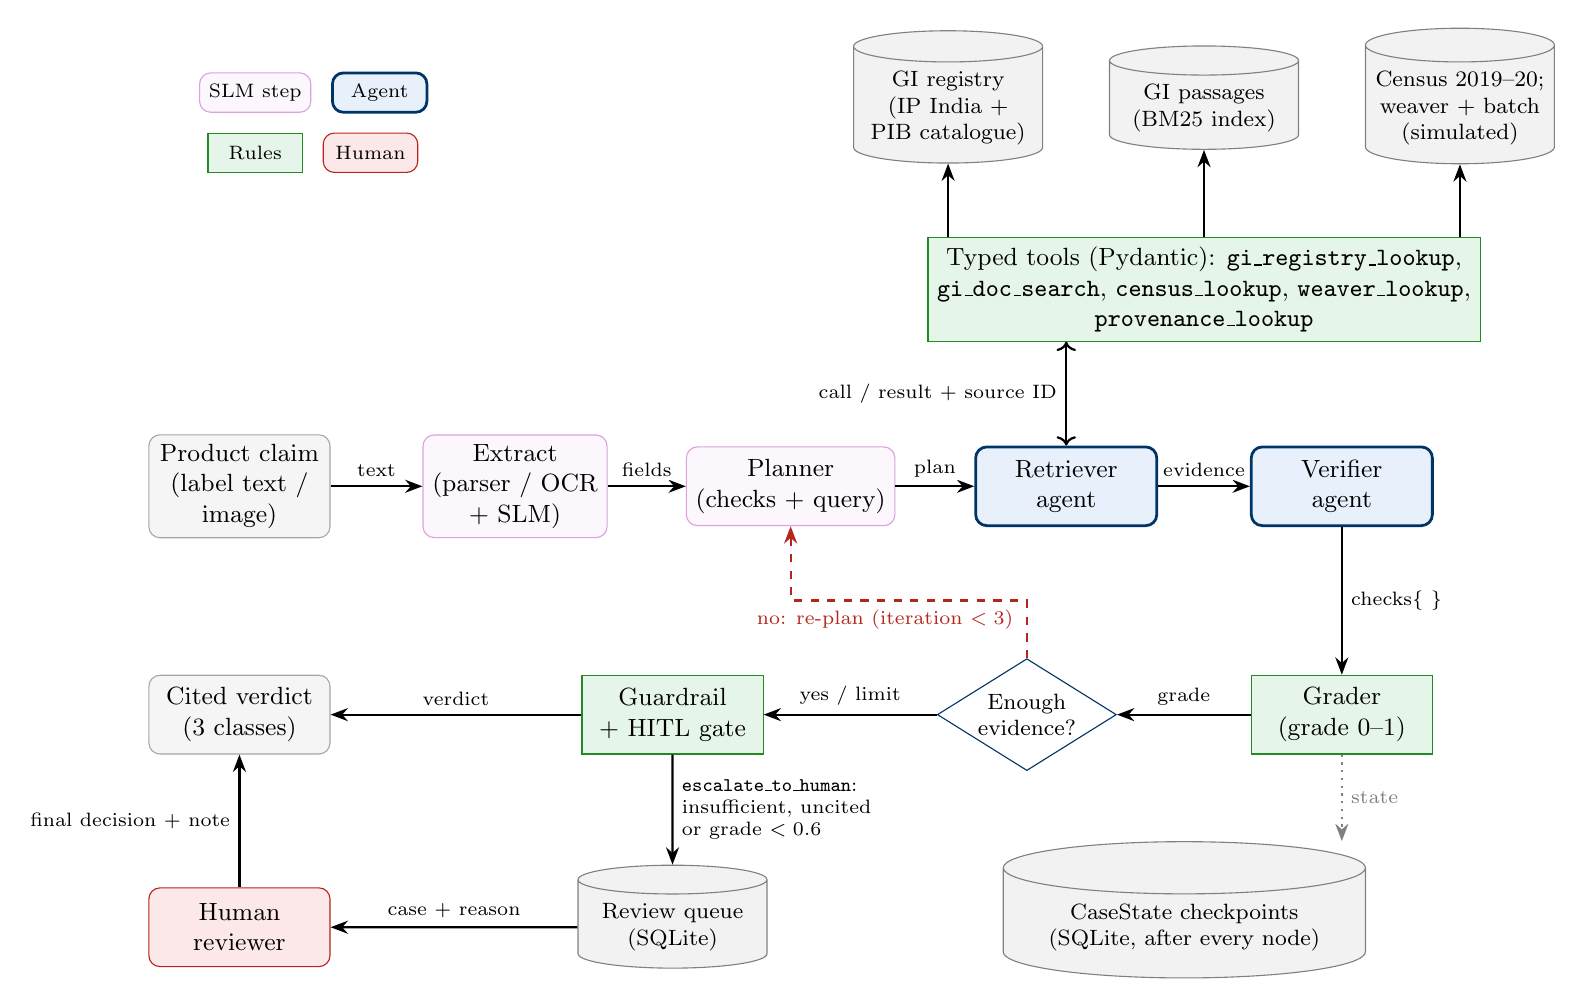
\begin{tikzpicture}[
  font=\small, every node/.append style={execute at begin node=\setstretch{1.0}},
  io/.style={draw=gray!70,fill=gray!8,rounded corners,minimum width=2.3cm,minimum height=1.0cm,align=center},
  slm/.style={draw=Plum,fill=Plum!8,rounded corners,minimum width=2.3cm,minimum height=1.0cm,align=center},
  agent/.style={draw=bmsblue,fill=guidebg,rounded corners,line width=1pt,minimum width=2.3cm,minimum height=1.0cm,align=center},
  rule/.style={draw=ForestGreen,fill=dobg,minimum width=2.3cm,minimum height=1.0cm,align=center},
  tool/.style={draw=ForestGreen,fill=dobg,minimum width=5.6cm,minimum height=1.0cm,align=center},
  store/.style={draw=gray,fill=gray!10,cylinder,shape border rotate=90,aspect=0.18,minimum width=2.4cm,minimum height=1.1cm,align=center,font=\footnotesize},
  human/.style={draw=BrickRed,fill=dontbg,rounded corners,minimum width=2.3cm,minimum height=1.0cm,align=center},
  dec/.style={draw=bmsblue,fill=white,diamond,aspect=1.6,inner sep=1pt,align=center,font=\footnotesize},
  arr/.style={-{Stealth[length=2.2mm]},thick},
  lab/.style={font=\scriptsize,fill=white,inner sep=1pt}]

% data stores (top)
\node[store] (reg) at (9.0,4.8) {GI registry\\(IP India +\\PIB catalogue)};
\node[store] (docs) at (12.25,4.8) {GI passages\\(BM25 index)};
\node[store] (cen) at (15.5,4.8) {Census 2019--20;\\weaver + batch\\(simulated)};
% tools
\node[tool,minimum width=6.8cm] (tools) at (12.25,2.5) {Typed tools (Pydantic): \texttt{gi\_registry\_lookup},\\\texttt{gi\_doc\_search}, \texttt{census\_lookup}, \texttt{weaver\_lookup},\\\texttt{provenance\_lookup}};
% main row
\node[io] (in) at (0,0) {Product claim\\(label text /\\image)};
\node[slm] (ext) at (3.5,0) {Extract\\(parser / OCR\\+ SLM)};
\node[slm] (plan) at (7.0,0) {Planner\\(checks + query)};
\node[agent] (ret) at (10.5,0) {Retriever\\agent};
\node[agent] (ver) at (14.0,0) {Verifier\\agent};
% second row
\node[rule] (gr) at (14.0,-2.9) {Grader\\(grade 0--1)};
\node[dec] (dec) at (10.0,-2.9) {Enough\\evidence?};
\node[rule] (gd) at (5.5,-2.9) {Guardrail\\+ HITL gate};
\node[io] (out) at (0,-2.9) {Cited verdict\\(3 classes)};
% third row
\node[store] (q) at (5.5,-5.6) {Review queue\\(SQLite)};
\node[human] (hum) at (0,-5.6) {Human\\reviewer};
\node[store,minimum width=4.6cm] (cp) at (12.0,-5.6) {CaseState checkpoints\\(SQLite, after every node)};

% arrows main flow
\draw[arr] (in) -- node[lab,above=2pt]{text} (ext);
\draw[arr] (ext) -- node[lab,above=2pt]{fields} (plan);
\draw[arr] (plan) -- node[lab,above=2pt]{plan} (ret);
\draw[arr] (ret) -- node[lab,above=2pt]{evidence} (ver);
\draw[arr] (ver) -- node[lab,right=2pt]{checks\{ \}} (gr);
\draw[arr] (gr) -- node[lab,above=2pt]{grade} (dec);
\draw[arr] (dec) -- node[lab,above=2pt]{yes / limit} (gd);
\draw[arr] (gd) -- node[lab,above=2pt]{verdict} (out);
\draw[arr,dashed,BrickRed] (dec.north) -- (dec.north |- 0,-1.45) -| node[lab,pos=0.3,below=2pt]{no: re-plan (iteration $<3$)} (plan.south);
% tools
\draw[arr,<->] (ret.north) -- node[lab,left=2pt]{call / result + source ID} (ret.north |- tools.south);
\draw[arr] (tools.north -| reg) -- (reg.south);
\draw[arr] (tools.north -| docs) -- (docs.south);
\draw[arr] (tools.north -| cen) -- (cen.south);
% HITL
\draw[arr] (gd) -- node[lab,right=2pt,align=left]{\texttt{escalate\_to\_human}:\\insufficient, uncited\\or grade $<0.6$} (q);
\draw[arr] (q) -- node[lab,above=2pt]{case + reason} (hum);
\draw[arr] (hum) -- node[lab,left=2pt]{final decision + note} (out);
% checkpoints
\draw[arr,dotted,gray] (gr.south) -- node[lab,right=2pt]{state} (gr.south |- cp.north);

% legend
\node[slm,minimum width=1.2cm,minimum height=0.5cm,font=\scriptsize] (l1) at (0.2,5.0) {SLM step};
\node[agent,minimum width=1.2cm,minimum height=0.5cm,font=\scriptsize,right=0.25cm of l1] (l2) {Agent};
\node[rule,minimum width=1.2cm,minimum height=0.5cm,font=\scriptsize,below=0.25cm of l1] (l3) {Rules};
\node[human,minimum width=1.2cm,minimum height=0.5cm,font=\scriptsize,right=0.25cm of l3] (l4) {Human};
\end{tikzpicture}}
\caption{Architecture of LoomTrace: six-node state graph, tools, data stores and human review}
\label{fig:arch}
\end{figure}

\section{Component Description}

Each component in Figure~\ref{fig:arch} is described below in terms of its responsibility, its inputs
and outputs, the method it uses, and its behaviour on failure.

\subsection{Product Claim Input and Extract Node}

The input is the text of a product label or seller claim, optionally accompanied by a label image. The
\emph{Extract} node calls the \texttt{extract\_label} tool, which produces a typed \texttt{LabelFields}
object with the fields \texttt{product}, \texttt{region}, \texttt{state}, \texttt{material},
\texttt{weaver\_id}, \texttt{batch\_id} and a Boolean \texttt{gi\_claim}. If an image is provided and the
EasyOCR package~\cite{easyocr} is installed, the image text is recognised first. If an API key is
configured, a small language model (SLM), Llama~3.1~8B~\cite{llama3}, is asked to return the fields as
JSON. Otherwise, and whenever the model call fails, a deterministic parser reads ``key: value'' lines,
recognises identifier patterns such as \texttt{WV-KAN-001} and \texttt{B-KAN-0010}, and falls back to
searching the text for known product names. Missing fields are left empty rather than guessed, so that
later nodes can treat them as unknown.

\subsection{Planner}

The planner decides which checks the claim requires and what to search for. Three checks are always
planned (product registered, GI document support and census plausibility); region, state and material
checks are planned only when the corresponding field is present; and four producer checks (weaver
registered, weaver in the correct cluster, batch found, batch woven by the claimed weaver) are always
planned so that their absence is visible. On the first iteration the planner requests an exact match in
the registry and an unfiltered document search using the product name and region as the query. On a
re-plan it resolves the product name to its registered form by matching the longest known alias, and
builds a sharper query from the canonical name, region, state, registered materials and words that
occur in statements of case (``geographical area weavers woven''), filtered to that product. If the
product cannot be resolved, the second iteration records the product check as failed rather than
looping indefinitely.

\subsection{Retriever Agent and Tools}

The retriever agent executes the plan by calling the tools listed in Table~\ref{tab:tools} in
Chapter~6: \texttt{gi\_registry\_lookup}, \texttt{gi\_doc\_search}, \texttt{census\_lookup} and, when the
identifiers are present, \texttt{weaver\_lookup} and \texttt{provenance\_lookup}. Every tool returns a
typed \texttt{ToolResult} containing a success flag, the data, a source identifier, a note and the
elapsed time. The retriever appends each result to the evidence list in the state, tagged with the
iteration number. Tool failures, such as an unknown weaver identifier, are returned as results with
\texttt{ok=false} and an explanatory note; they are never raised as exceptions, so that the verifier can
reason about them.

\subsection{Verifier Agent}

The verifier agent judges the evidence of the current iteration. It runs up to ten rule-based checks
and assigns each a status of \emph{pass}, \emph{fail} or \emph{unknown}, together with a plain-language
reason and the source identifier on which the status rests. For example, the region check passes if
the claimed region matches one of the registered districts, fails if it does not, and is unknown if
the product could not be resolved; for GIs registered for a whole state, such as Muga Silk, the check
compares the state instead. A claimed weaver who is not in the registry yields \emph{unknown} for the
batch--weaver match rather than \emph{fail}, because a mismatch cannot be established against an
unverified identity. Deterministic rules are used for these checks because they are exact and
repeatable, which a small model is not.

\subsection{Grader}

The grader scores the evidence before any verdict is produced. It computes completeness $C$, the
fraction of checks that are not unknown, and the citation fraction $Q$, the fraction of determinate
checks that carry a source identifier. If no check has failed, the grade is $g = 0.7C + 0.3Q$; if a
check has failed, the grade is $g = 0.5 + 0.5Q$, because a cited contradiction is strong evidence even
when other checks are incomplete. The grader then decides whether to loop: it requests a re-plan if the
product check or the document-support check is unknown, a product name is present, and fewer than three
iterations have been used. Otherwise it passes control to the guardrail.

\subsection{Guardrail and Human Review Gate}

The guardrail converts the checks into a verdict: \emph{Conflicting evidence} if any check failed,
\emph{Insufficient evidence} if any check is unknown, and \emph{Supported} only if every check passed.
It then enforces two conditions: a decided verdict must have at least one citation, and its grade must
be at least 0.6; if either condition fails, the verdict is downgraded to \emph{Insufficient evidence}.
Every \emph{Insufficient evidence} verdict is passed to the \texttt{escalate\_to\_human} tool, which
inserts the case, the extracted claim and the reason (for example, ``missing: weaver\_registered,
batch\_found'') into the review queue. The guardrail also writes the case to the case history.

\subsection{Review Queue and Human Reviewer}

The review queue is a table in the SQLite database. A reviewer sees each open case with its details
and reason, writes a note, and records one of three decisions (confirm authentic, not authentic, cannot
confirm). The decision is stored in a separate table and becomes the final verdict for the case, and
the requester can see it, with the note, by entering the case reference. A requester can also send a
case that was decided automatically to the queue if they disagree with the result.

\subsection{Data Stores and Checkpoints}

The four data stores are the GI registry (fifteen products), the GI passage index (21 passages), the
census table (31 rows) and the simulated weaver and batch records (180 and 360 records), described in
Section~3.4. The \texttt{CaseState} checkpoint store is an SQLite table to which the full state is
written after every node, giving each case its own memory and a durable history.

\section{Selected Agentic Patterns and Justification}

Table~\ref{tab:patterns} lists the patterns used, where each is applied, why it was chosen and which
alternative was rejected.

\begin{table}[H]
\centering
\caption{Agentic patterns and design justification}
\label{tab:patterns}
\small
\begin{tabularx}{\linewidth}{@{}>{\raggedright\arraybackslash}p{2.4cm} >{\raggedright\arraybackslash}p{2.4cm} >{\raggedright\arraybackslash}X >{\raggedright\arraybackslash}p{3.0cm}@{}}
\toprule
\textbf{Pattern} & \textbf{Where} & \textbf{Reason} & \textbf{Alternative rejected} \\ \midrule
Tool use & Retriever agent & Facts must come from registry, census and producer records, each with a source identifier & Answering from model memory \\
Agentic (corrective) RAG & Planner, retriever, grader & Labels use aliases; a weak first search must be detected and repeated with a sharper, filtered query~\cite{yan2024crag} & Single-shot retrieval \\
Plan-and-execute with re-planning & Planner, grader loop & Applicable checks depend on which fields are present; steps are known, so they can be bounded and traced~\cite{wang2023plansolve} & Free-form ReAct loop~\cite{yao2023react} \\
Supervisor multi-agent & Graph routes between retriever and verifier & One narrow responsibility per node: gathering evidence is separated from judging it & One node doing both \\
Reflection (evidence grading) & Grader & Verdicts must not be issued on incomplete evidence~\cite{shinn2023reflexion} & No self-check \\
HITL and guardrails & Guardrail, review queue & A wrong verdict harms a producer or a buyer; abstention is safer than a guess & Fully automatic decision \\
\bottomrule
\end{tabularx}
\end{table}

The main design decision was to use an explicit graph with deterministic checks rather than a
free-form ReAct agent. In a free-form agent, the model chooses which tool to call next and when to stop,
which makes the number of steps unbounded and the trace harder to audit. In LoomTrace the sequence of
nodes is fixed, only the plan contents and the loop decision vary, and the loop has a hard limit. A
second decision was to keep model calls narrow. Small models are fast and inexpensive but are weaker at
long, open-ended reasoning~\cite{liu2024lost}; giving the model only extraction and explanation, while
rules perform the factual checks, keeps the system correct even when no model is available.

\section{Control Flow and Agent State}

Control moves through the graph as follows. The graph starts at \emph{Extract}, then runs
\emph{Planner}, \emph{Retriever}, \emph{Verifier} and \emph{Grader} in sequence. A conditional edge
after the grader routes to the planner when the grader's decision is ``re-plan'' and to the guardrail
when it is ``finish''; the guardrail leads to the end of the graph. The loop terminates under exactly
three conditions: (i) the product and document checks are both determinate; (ii) no product name was
extracted, so re-planning cannot help; or (iii) the iteration counter has reached the limit of three
iterations. In addition, LangGraph's recursion limit is set to 40 node executions as a second,
independent bound. A full run without re-planning executes 6 nodes, and each re-plan adds 4 nodes.

Table~\ref{tab:state} lists the fields of the shared state.

\begin{table}[H]
\centering
\caption{Fields of the shared CaseState}
\label{tab:state}
\small
\begin{tabularx}{\linewidth}{@{}>{\ttfamily}l >{\raggedright\arraybackslash}X >{\raggedright\arraybackslash}p{2.6cm}@{}}
\toprule
\normalfont\textbf{Field} & \textbf{Content} & \textbf{Written by} \\ \midrule
case\_id & Unique reference, e.g.\ \texttt{CASE-94767A68} & Input \\
label\_text, image & Raw claim text and optional image bytes & Input \\
fields & Extracted \texttt{LabelFields} & Extract \\
plan, query, resolve\_aliases & Checks to run, search query, alias-resolution flag & Planner \\
canonical & Registered product name, once resolved & Retriever \\
evidence[ ] & Tool results with source IDs and iteration (append-only) & All tool-calling nodes \\
checks\{ \} & Status, reason and source per check & Verifier \\
grade, grade\_detail & Score 0--1, completeness, consistency, decision & Grader \\
iteration & Planning iterations used (0--2) & Extract, Grader \\
verdict, confidence, citations, rationale & Final output & Guardrail \\
escalated & Review-queue entry, if any & Guardrail \\
trace[ ] & One entry per node with a summary message (append-only) & All nodes \\
\bottomrule
\end{tabularx}
\end{table}

The \texttt{evidence} and \texttt{trace} fields are declared with an additive reducer, so that each
node appends to them instead of replacing them. This preserves the evidence of every iteration and
makes the full history of a case available to the verifier, the interface and the checkpoint store.

\section{Data Flow}

The following example traces one real input through the system. The label reads ``Product: Kanjivaram
Silk Saree; Region: Thiruvallur; State: Tamil Nadu; Material: mulberry silk; Weaver ID: WV-KAN-001;
Batch ID: B-KAN-0010''.

\begin{enumerate}[itemsep=2pt]
\item \textbf{Extract} produces the six fields; the product is the alias ``Kanjivaram Silk Saree''.
\item \textbf{Planner (iteration 0)} plans ten checks and the query ``Kanjivaram Silk Saree
Thiruvallur'', with exact registry matching.
\item \textbf{Retriever} calls five tools. The registry lookup fails (no exact match); the document
search returns five passages, two from the Kancheepuram corpus and three from other products; the
census, weaver and batch lookups succeed.
\item \textbf{Verifier} reports 5 pass, 0 fail and 5 unknown: the product, region, state, material and
cluster checks cannot be made without a registry entry.
\item \textbf{Grader} computes completeness 0.5 and citation fraction 1.0, so $g = 0.65$; because the
product check is unknown, it requests a re-plan.
\item \textbf{Planner (iteration 1)} resolves the alias to ``Kancheepuram Silk'' and issues a query
filtered to that product.
\item \textbf{Retriever} now finds registry entry GI~15 and three Kancheepuram passages.
\item \textbf{Verifier} reports 10 pass, 0 fail, 0 unknown; \textbf{Grader} computes $g = 1.0$ and
finishes.
\item \textbf{Guardrail} issues \emph{Supported} with seven citations: three GI passages, the registry
entry, the Tamil Nadu census row, and the weaver and batch records.
\end{enumerate}

The case executed ten nodes, made eleven tool calls and wrote ten checkpoints. The complete trace of
this run is given in Listing~\ref{lst:replan} in Chapter~5.

%---------------------------------------------------------------------
\chapter{Agentic Concepts Demonstrated}
%---------------------------------------------------------------------

This chapter maps LoomTrace to the agentic-concept checklist of the course. All five mandatory
concepts are implemented. Of the five bonus concepts, two are fully implemented and three are
implemented in part; the partial ones are stated as such. Every item is supported by evidence from a
real run: a trace excerpt, a tool log, a screenshot or a section of this report. All traces in this
chapter were produced by the system on 11 November 2026 and are reproduced without editing, except
that long lines are wrapped and non-ASCII symbols (tick, cross, arrow and middle dot) are replaced by
the ASCII equivalents OK, X, \texttt{->} and a full stop.

\section{Concept Coverage Matrix}

Table~\ref{tab:coverage} summarises the coverage.

\begin{table}[H]
\centering
\caption{Coverage of the agentic-concept checklist}
\label{tab:coverage}
\small
\begin{tabularx}{\linewidth}{@{}l >{\raggedright\arraybackslash}p{3.6cm} c >{\raggedright\arraybackslash}X@{}}
\toprule
\textbf{Tier} & \textbf{Concept} & \textbf{Status} & \textbf{Evidence} \\ \midrule
Mandatory & Tool / function use & \checkmark & Seven typed tools; Listing~\ref{lst:tools}, Table~\ref{tab:tools} \\
Mandatory & Agentic RAG & \checkmark & Weak first retrieval detected and repeated with a filtered query; Listings~\ref{lst:replan}, \ref{lst:tools} \\
Mandatory & Planning and reasoning & \checkmark & Planner output and re-plan in Listing~\ref{lst:replan}; Algorithm~\ref{alg:loop} \\
Mandatory & Observability / tracing & \checkmark & Node trace and per-node SQLite checkpoints; Section~7.1, Listing~\ref{lst:ckpt} \\
Mandatory & Evaluation & \checkmark & 45-case labelled set, baseline comparison; Chapter~7 \\
Bonus & Multi-agent collaboration & Partial & Separate retriever and verifier nodes routed by the graph (supervisor); both are deterministic, not independent model agents \\
Bonus & Memory & Partial & Per-case memory in CaseState and checkpoint history; no memory across cases \\
Bonus & Human-in-the-loop and guardrails & \checkmark & Guardrail, review queue, reviewer decisions; Listing~\ref{lst:hitl}, Figs.~\ref{fig:admin}, \ref{fig:track} \\
Bonus & Durable workflow & Partial & Full state persisted after every node; automatic resumption from a checkpoint is not implemented \\
Bonus & Experimentation & \checkmark & A/B experiment on the re-planning loop; Chapter~8 \\
\bottomrule
\end{tabularx}
\end{table}

\section{Evidence for Each Concept}

\subsection{Tool Use}

Listing~\ref{lst:tools} shows the tool log of the run described in Section~4.5, as stored in the
\texttt{evidence} field of the state. Each line gives the planning iteration, the tool name, whether it
succeeded, the source identifier it returned and its note. In iteration~0 the registry lookup fails
because ``Kanjivaram Silk Saree'' is not the registered name, while the other tools succeed. In
iteration~1 the same tools are called with the resolved product, and the registry returns entry GI~15.
Simulated records are marked as such in the tool output itself.

\begin{lstlisting}[language={},caption={Tool calls for the Kanjivaram case (iteration, tool, ok, source ID, note)},label={lst:tools}]
-  extract_label      True   LABEL#input                   parsed label text
0  gi_registry_lookup False  None   'Kanjivaram Silk Saree' not found (exact match)
0  gi_doc_search      True   GI15-p3,GI15-p5,PIB-GI-2021-p4,PIB-GI-2021-p7,
                             PIB-GI-2021-p12               5 passages (unfiltered)
0  census_lookup      True   HLCENSUS-2019-20#Tamil_Nadu
0  weaver_lookup      True   SIM-WEAVER#WV-KAN-001         SIMULATED record
0  provenance_lookup  True   SIM-PROV#B-KAN-0010           SIMULATED record
1  gi_registry_lookup True   IPINDIA-GI-REG#15
1  gi_doc_search      True   GI15-p3,GI15-p5,GI15-p7       3 passages filtered to
                                                           Kancheepuram Silk
1  census_lookup      True   HLCENSUS-2019-20#Tamil_Nadu
1  weaver_lookup      True   SIM-WEAVER#WV-KAN-001         SIMULATED record
1  provenance_lookup  True   SIM-PROV#B-KAN-0010           SIMULATED record
\end{lstlisting}

\subsection{Agentic RAG}

Retrieval in LoomTrace is agentic in the sense used by corrective RAG~\cite{yan2024crag}: the result
of retrieval is evaluated, and a poor result changes what the agent does next. In
Listing~\ref{lst:tools}, the unfiltered search in iteration~0 returns five passages, of which only two
belong to Kancheepuram Silk; the other three describe other products. Because the registry did not
resolve the product, the grader marks the evidence as insufficient. The planner then rewrites the
query using the canonical name, the region, the state and the registered materials, and restricts the
search to the resolved product; the second search returns three passages, all from the Kancheepuram
corpus. The verdict cites these passages, so every \emph{Supported} or \emph{Conflicting} verdict is
grounded in official text about the specific product.

\subsection{Planning and Reasoning}

Listing~\ref{lst:replan} shows the node-level trace of the same run. The planner first produces an
initial plan of ten checks with exact matching. After the verifier finds five checks unknown, the
grader computes a grade of 0.65 with completeness 0.5 and requests a re-plan. The second plan resolves
the alias, after which all ten checks pass and the grader finishes with a grade of 1.0. The reasoning
over the evidence is explicit in the verifier's per-check reasons, for example ``Region `Thiruvallur'
is in GI area (Kancheepuram, Thiruvallur)''.

\begin{lstlisting}[language={},caption={Node trace showing evidence grading and re-planning (case REPORT-TRACE-1)},label={lst:replan}]
{"node": "Extract",   "msg": "parsed label text: product=Kanjivaram Silk Saree,
   region=Thiruvallur, state=Tamil Nadu, weaver_id=WV-KAN-001,
   batch_id=B-KAN-0010, material=mulberry silk"}
{"node": "Planner",   "msg": "Initial plan: exact registry match, unfiltered
   document search"}
{"node": "Retriever", "msg": "gi_registry_lookup X . gi_doc_search OK .
   census_lookup OK . weaver_lookup OK . provenance_lookup OK"}
{"node": "Verifier",  "msg": "5 pass . 0 fail . 5 unknown"}
{"node": "Grader",    "msg": "grade=0.65 (completeness 0.5, consistency 1.0)
   -> re-plan"}
{"node": "Planner",   "msg": "Re-plan #1: resolve aliases -> 'Kancheepuram Silk',
   sharper query filtered by product"}
{"node": "Retriever", "msg": "gi_registry_lookup OK . gi_doc_search OK .
   census_lookup OK . weaver_lookup OK . provenance_lookup OK"}
{"node": "Verifier",  "msg": "10 pass . 0 fail . 0 unknown"}
{"node": "Grader",    "msg": "grade=1.0 (completeness 1.0, consistency 1.0)
   -> finish"}
{"node": "Guardrail", "msg": "Supported"}
\end{lstlisting}

\subsection{Observability}

Every node appends one entry to the \texttt{trace} field, and every tool result is kept in the
\texttt{evidence} field with its timing in milliseconds. In addition, a wrapper around each node writes
the complete state to the \texttt{checkpoints} table in SQLite after the node finishes.
Listing~\ref{lst:ckpt} shows the checkpoint rows for the run above: ten rows, one per executed node,
with the second planning iteration visible as steps 5--8. Section~7.1 describes what is recorded in
more detail. The project's design document proposed LangSmith for tracing; it was not used, because
the local trace and checkpoint store provide the same per-node visibility without an external account,
and they can be queried with SQL.

\begin{lstlisting}[language={},caption={Checkpoint rows (step, node) stored for case REPORT-TRACE-1},label={lst:ckpt}]
(0,'extract') (1,'planner') (2,'retriever') (3,'verifier') (4,'grader')
(5,'planner') (6,'retriever') (7,'verifier') (8,'grader') (9,'guardrail')
\end{lstlisting}

\subsection{Evaluation}

Quality is measured on a labelled set of 45 cases with exact-match metrics, a single-lookup baseline
and per-class precision, recall and F1-score, as reported in Chapter~7. A separate set of 15
hand-written demonstration cases covering nine products is reported in Section~7.5.

\subsection{Bonus Concepts}

\paragraph{Human-in-the-loop and guardrails.} Listing~\ref{lst:hitl} shows a run in which the label
contains no weaver or batch identifier. The verifier marks four producer checks as unknown, the grader
finishes because re-planning cannot supply missing identifiers, and the guardrail escalates the case to
the review queue with the reason stated. Figure~\ref{fig:admin} shows the reviewer dashboard with such
a case awaiting a decision, and Figure~\ref{fig:track} shows the requester's view after a reviewer
confirmed the claim with a note.

\begin{lstlisting}[language={},caption={Trace of an abstention and escalation (case REPORT-TRACE-2)},label={lst:hitl}]
{"node": "Extract",   "msg": "parsed label text: product=Banaras Brocades and
   Sarees, region=Varanasi, state=Uttar Pradesh"}
{"node": "Planner",   "msg": "Initial plan: exact registry match, unfiltered
   document search"}
{"node": "Retriever", "msg": "gi_registry_lookup OK . gi_doc_search OK .
   census_lookup OK"}
{"node": "Verifier",  "msg": "5 pass . 0 fail . 4 unknown"}
{"node": "Grader",    "msg": "grade=0.69 (completeness 0.56, consistency 1.0)
   -> finish"}
{"node": "Guardrail", "msg": "Insufficient evidence -> escalated to human
   (queue #183)"}
reason: "missing: weaver_registered, weaver_cluster, batch_found,
         batch_weaver_match"
\end{lstlisting}

\begin{figure}[H]
\centering
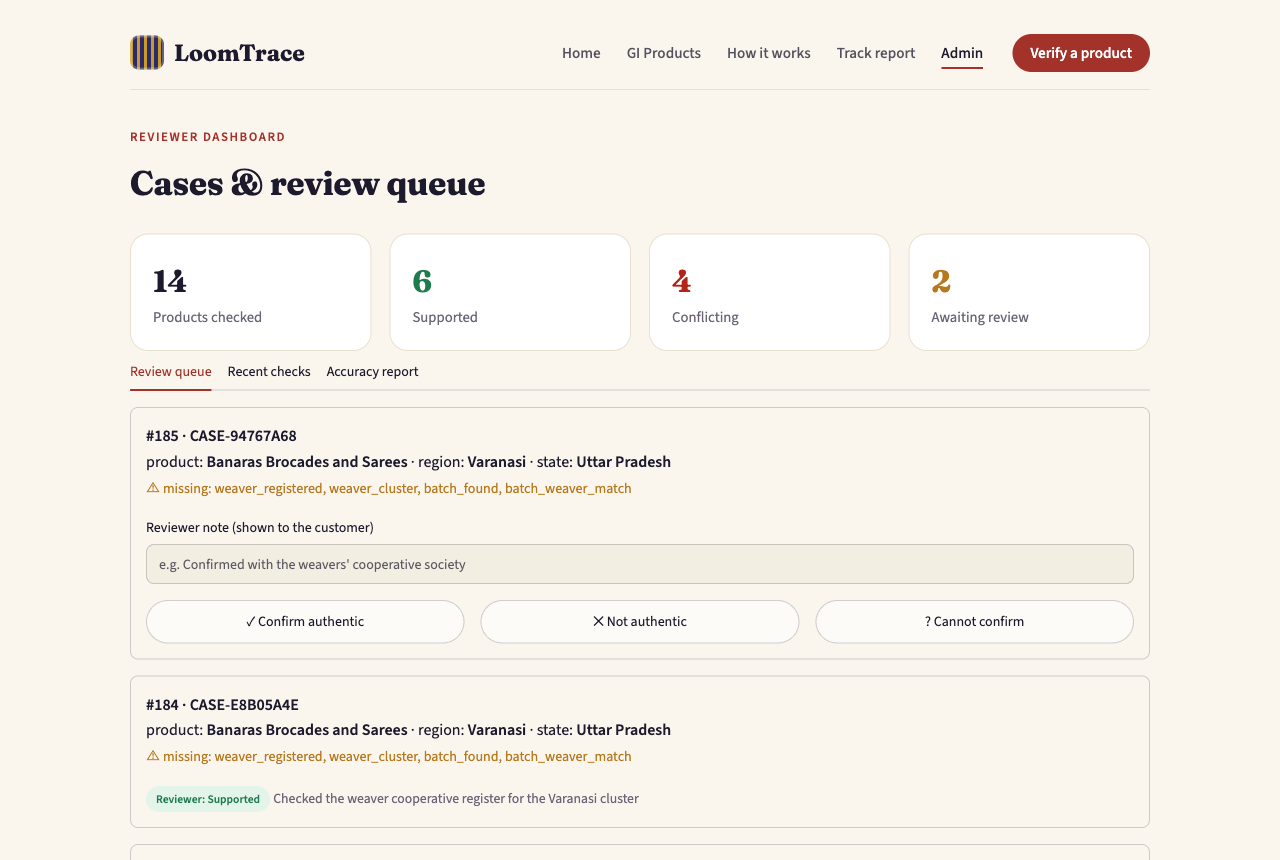
\includegraphics[width=0.8\linewidth]{figures/ui_admin.png}
\caption{Reviewer dashboard: open case with extracted claim, escalation reason, note field and
decision buttons; below it, an earlier case already decided by a reviewer}
\label{fig:admin}
\end{figure}

\begin{figure}[H]
\centering
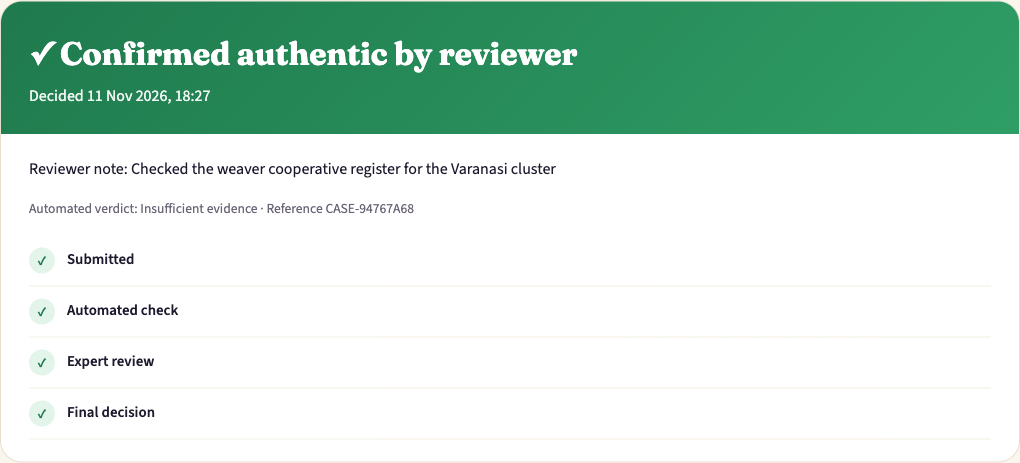
\includegraphics[width=0.5\linewidth]{figures/ui_track.png}
\caption{Requester's view of an escalated case after the reviewer's decision, with the reviewer's
note, the automated verdict and the progress of the case}
\label{fig:track}
\end{figure}

\paragraph{Multi-agent collaboration (partial).} Gathering evidence and judging it are performed by two
separate nodes, the retriever agent and the verifier agent, and the graph's conditional routing acts as
a supervisor. Both nodes are deterministic in the configuration evaluated, so this is a division of
responsibilities rather than a collaboration of independent model-driven agents.

\paragraph{Memory (partial).} Each case has its own memory: the CaseState accumulates the evidence and
trace of every iteration, the checkpoint table preserves each intermediate state, and the case history
and decision tables keep the outcome. There is no memory across cases; for example, the system does
not learn that a particular seller's claims are frequently escalated.

\paragraph{Durable workflow (partial).} Because the full state is written after every node, a case can be
inspected and re-checked at any later time, and human review proceeds asynchronously through the queue.
However, the graph does not automatically resume an interrupted run from its last checkpoint; a run
that is interrupted is re-executed from the start.

\paragraph{Experimentation.} Chapter~8 reports a controlled A/B experiment in which the re-planning loop
is disabled while all other factors are held fixed.

%---------------------------------------------------------------------
\chapter{Implementation}
%---------------------------------------------------------------------

This chapter describes how the design of Chapter~4 was built: the technology stack, the preparation
of the reference data and the retrieval index, the agent loop, the tools, the prompts, the guardrails
and loop bounds, the user interface and the repository structure. Together with
Appendix~\ref{app:run}, it is intended to allow another student to reproduce the system.

\section{Technology Stack}

Table~\ref{tab:stack} lists the technologies used, with the exact versions installed in the project's
virtual environment.

\begin{table}[H]
\centering
\caption{Technology stack}
\label{tab:stack}
\small
\begin{tabularx}{\linewidth}{@{}>{\raggedright\arraybackslash}p{3.4cm} >{\raggedright\arraybackslash}p{4.4cm} >{\raggedright\arraybackslash}X@{}}
\toprule
\textbf{Layer} & \textbf{Choice (version)} & \textbf{Reason} \\ \midrule
Language & Python 3.13.7 & Standard for agent tooling \\
Orchestration & LangGraph 1.2.20~\cite{langgraph} & Explicit state graph with conditional edges and reducers \\
Schemas & Pydantic 2.14.3~\cite{pydantic} & Typed tool inputs and outputs, validated at run time \\
Language model (optional) & Llama~3.1~8B Instant~\cite{llama3} via Groq API, client 1.7.0~\cite{groq} & Small, fast model with JSON output; free tier \\
Retrieval & BM25~\cite{robertson2009bm25}, implemented in Python & Transparent keyword ranking over a small official corpus \\
OCR (optional) & EasyOCR~\cite{easyocr} & Label images; not installed for the reported runs \\
Persistence & SQLite~\cite{sqlite} (Python \texttt{sqlite3}) & Checkpoints, review queue, decisions, case history \\
Interface & Streamlit 1.67.0~\cite{streamlit} with custom HTML and CSS & Web pages for requesters and reviewers \\
Tables & pandas 3.1.1 & Reviewer and evaluation tables \\
\bottomrule
\end{tabularx}
\end{table}

The design document proposed Chroma with \texttt{bge-small} embeddings as the vector store. This was
replaced by BM25 because the corpus contains only 21 short passages whose relevant terms (district
names, materials, product names) are exact keywords, for which lexical matching is reliable, and
because BM25 needs no model download, so the evaluation runs offline and deterministically. Dense
retrieval would become preferable if the full scanned GI applications were indexed (Section~10.2).

\section{Data Preparation and Indexing}

\paragraph{Registry.} Each of the fifteen products is stored as a record with its GI application number
(where known), state, goods class, list of registered districts or places, list of aliases, registered
materials, a \texttt{state\_wide} flag and a source identifier. Aliases were written by the team from
common market names, for example ``kanjivaram'', ``kanjeevaram'' and ``kanchi pattu'' for Kancheepuram
Silk. When several aliases match a label, the longest match is chosen, so that ``Sambalpuri ikat''
resolves to Sambalpuri Bandha rather than to Pochampalli Ikat through the shorter alias ``ikat''.

\paragraph{Census.} The 31 rows of the PIB annexure were transcribed into a table of state, weavers and
allied workers, keyed by state name. The All-India total in the source (26,73,891 weavers) was used to
check the transcription.

\paragraph{Retrieval corpus and index.} The corpus has 21 passages: three for each of the three
original products and one for each of the twelve catalogue products, the latter taken from the
description in the PIB GI catalogue. Each passage carries its product and a page reference as metadata.
Documents are not chunked further, because each passage is a single paragraph of 20 to 59 words that
describes one aspect of one product; splitting would separate district names from the product they
refer to. Text is lower-cased and tokenised into alphabetic words, the product name is appended to
each passage, and BM25 statistics (document frequencies and average length) are computed once at
start-up. Scoring uses the standard parameters $k_1 = 1.5$ and $b = 0.75$:
\begin{equation}
\mathrm{score}(q,d) = \sum_{t \in q} \mathrm{IDF}(t)\,\frac{f(t,d)\,(k_1+1)}{f(t,d) + k_1\left(1 - b + b\,\frac{|d|}{\overline{|d|}}\right)},
\end{equation}
where $f(t,d)$ is the frequency of term $t$ in passage $d$ and
$\mathrm{IDF}(t) = \ln\!\left(1 + \frac{N - n_t + 0.5}{n_t + 0.5}\right)$ for $N$ passages of which
$n_t$ contain $t$. The search returns at most five passages with a score above zero, optionally
restricted to one product. A first-iteration search is considered adequate evidence only if its top
score is at least 2.0. This value was fixed by the team during development as a conservative
minimum and was not tuned on the test set; once the product has been resolved through the registry,
any passage retrieved for that product is accepted as document support.

\paragraph{Simulated producer records.} The generator described in Section~3.4 is run at import time with
a fixed seed, producing identifiers of the form \texttt{WV-KAN-001} for weavers and
\texttt{B-KAN-0010} for batches, where the three-letter code identifies the product.

\section{Core Agent Loop}

Algorithm~\ref{alg:loop} gives the agent loop in pseudocode.

\begin{algorithm}[H]
\caption{LoomTrace agent loop}
\label{alg:loop}
\begin{algorithmic}[1]
\Require claim text $x$, maximum iterations $L = 3$
\State $f \gets \textsc{Extract}(x)$; \quad $i \gets 0$; \quad $E \gets [\,]$
\Loop
  \State $(P, q, \mathit{resolve}) \gets \textsc{Plan}(f, i)$ \Comment{checks, query, alias flag}
  \State $E \gets E \cup \textsc{Retrieve}(f, q, \mathit{resolve})$ \Comment{tool calls, tagged with $i$}
  \State $C \gets \textsc{Verify}(f, E_i)$ \Comment{pass / fail / unknown per check}
  \State $g \gets \textsc{Grade}(C)$
  \If{$\textsc{Unresolved}(C) \land f.\mathit{product} \neq \varnothing \land i + 1 < L$}
    \State $i \gets i + 1$ \Comment{re-plan}
  \Else
    \State \textbf{break}
  \EndIf
\EndLoop
\State $v \gets$ \textsc{Conflicting} \textbf{if} any $c \in C$ fails \textbf{else} \textsc{Insufficient} \textbf{if} any is unknown \textbf{else} \textsc{Supported}
\If{$v \neq \textsc{Insufficient} \land (\textsc{Citations}(C) = \varnothing \lor g < 0.6)$}
  \State $v \gets \textsc{Insufficient}$ \Comment{guardrail downgrade}
\EndIf
\If{$v = \textsc{Insufficient}$} \State \textsc{EscalateToHuman}$(x, f, \textsc{Reason}(C))$ \EndIf
\State \Return $v$, $\textsc{Citations}(C)$, $g$
\end{algorithmic}
\end{algorithm}

Line~1 extracts the fields and initialises the iteration counter and the evidence list. Lines~3--6 are
one planning iteration: the planner chooses the checks and query, the retriever calls the tools and
appends their results, the verifier evaluates only the evidence of the current iteration, and the
grader computes the grade. Line~7 is the loop condition: the agent re-plans only if the product or the
document evidence is still unresolved, a product name is available, and the limit of three iterations
has not been reached; otherwise the loop ends at line~10. Line~13 maps the checks to a verdict.
Lines~14--16 apply the guardrail, and lines~17--18 escalate every undecided case. In the
implementation, each line of the loop is a separate LangGraph node, the loop condition is a conditional
edge, and every node is wrapped by a function that writes a checkpoint after it runs.

\section{Tools and Function Definitions}

Table~\ref{tab:tools} lists the seven tools. Every tool returns a \texttt{ToolResult} object with the
fields \texttt{tool}, \texttt{ok}, \texttt{data}, \texttt{source\_id}, \texttt{note} and \texttt{ms}.

\begin{table}[H]
\centering
\caption{Tools available to the agent}
\label{tab:tools}
\small
\begin{tabularx}{\linewidth}{@{}>{\raggedright\arraybackslash}p{3.1cm} >{\raggedright\arraybackslash}p{4.1cm} >{\raggedright\arraybackslash}X@{}}
\toprule
\textbf{Tool} & \textbf{Input $\rightarrow$ output} & \textbf{Data source; error behaviour} \\ \midrule
\texttt{extract\_label} & Label text, optional image $\rightarrow$ \texttt{LabelFields} & EasyOCR and SLM if available, else rule parser; never fails, leaves fields empty \\
\texttt{gi\_registry\_lookup} & Product name, alias flag $\rightarrow$ GI no., state, districts, materials & Registry (IP India and PIB catalogue); \texttt{ok=false} with note if not found \\
\texttt{gi\_doc\_search} & Query, optional product $\rightarrow$ top-5 passages with scores and pages & BM25 index of 21 passages; \texttt{ok=false} if no passage scores above 0 \\
\texttt{census\_lookup} & State $\rightarrow$ weavers, allied workers & Census table (PIB annexure); \texttt{ok=false} for unknown state \\
\texttt{weaver\_lookup} & Weaver ID $\rightarrow$ name, cluster, district, looms & \textbf{Simulated} registry; \texttt{ok=false} for unknown ID \\
\texttt{provenance\_lookup} & Batch ID $\rightarrow$ weaver, loom, yarn, dates & \textbf{Simulated} records; \texttt{ok=false} for unknown ID \\
\texttt{escalate\_to\_human} & Case ID, reason, claim $\rightarrow$ queue entry & SQLite review queue; returns queue number \\
\bottomrule
\end{tabularx}
\end{table}

Two helper functions complete the human-review workflow: \texttt{decide}, which records a reviewer's
decision and note and closes the queue entry, and \texttt{case\_status}, which returns the automated
verdict, the queue entry and the reviewer's decision for a given case reference.

\section{Prompt Design}

The language model is used for two narrow tasks only, and both calls use temperature~0 and the JSON
output mode of the API. The extraction prompt asks for a fixed set of keys, requires \texttt{null} for
absent fields and requires identifiers to be copied exactly; the explanation prompt receives only the
verdict, the status of each check, and the source identifiers and notes of at most twelve tool results,
and is told to use only these and to cite sources in brackets. Both prompts are given in full in Appendix~\ref{app:prompts}. Restricting the model
to these inputs means that it cannot introduce facts that the tools did not return, and requiring JSON
means that malformed output is detected by parsing and replaced by the deterministic fall-back.

All evaluation results in this report were produced \emph{without} an API key, so the model was not
called and the deterministic parser and template explanations were used. The prompts have therefore not
been evaluated quantitatively, and no claim is made about the model's extraction accuracy.

\section{Guardrails and Loop Bounds}

The following guardrails are implemented, with their numerical values.

\begin{itemize}[itemsep=2pt]
\item \textbf{Iteration bound.} At most $L = 3$ planning iterations per case. In the evaluation, the
maximum observed was two iterations and eleven tool calls.
\item \textbf{Graph bound.} LangGraph recursion limit of 40 node executions per run, independent of the
iteration counter.
\item \textbf{Citation and confidence gate.} A \emph{Supported} or \emph{Conflicting} verdict requires
at least one citation and a grade of at least 0.6; otherwise it is downgraded to \emph{Insufficient
evidence}.
\item \textbf{Escalation.} Every \emph{Insufficient evidence} verdict is placed in the review queue.
\item \textbf{Typed input and output.} Extracted fields and tool results are validated by Pydantic
models; model output that does not parse as JSON is discarded.
\item \textbf{No guessing of identity.} An unknown weaver or batch identifier yields \emph{unknown}, not
\emph{fail}, so that a typing error does not produce a \emph{Conflicting} verdict.
\item \textbf{Coverage gate.} A product that does not resolve to one of the fifteen GIs is reported in the
interface as ``not covered'' before the agent runs, with an option to send it to a reviewer.
\item \textbf{Input handling.} Label text is treated only as data: it is parsed into fields and is never
executed or used to select tools.
\item \textbf{Output escaping and reviewer access.} Every user-supplied value (label fields, reasons and
reviewer notes) is HTML-escaped before it is displayed, so that text in a claim cannot inject markup
into the pages. The reviewer dashboard requires a password supplied through the environment variable
\texttt{LOOMTRACE\_ADMIN\_PASSWORD}, and decisions are recorded only for a signed-in reviewer.
\end{itemize}

\section{User Interface}

The interface is a Streamlit application styled as a website with five public pages (Home, GI Products,
How it works, Verify a product and Track report) and an Admin page for reviewers. On the Verify page
the requester enters the label fields or chooses an example, and the agent runs while a progress bar
shows plain-language status messages. The result is a report card, shown in Fig.~\ref{fig:ui}: a
coloured verdict header, the resolved product and GI status, the place of manufacture and the weaver,
the list of checks with a tick, cross or question mark and a reason for each, and the list of sources.
The reviewer dashboard and the tracking page were shown in Figs.~\ref{fig:admin} and~\ref{fig:track}.

\begin{figure}[H]
\centering
\begin{minipage}[t]{0.48\linewidth}\centering
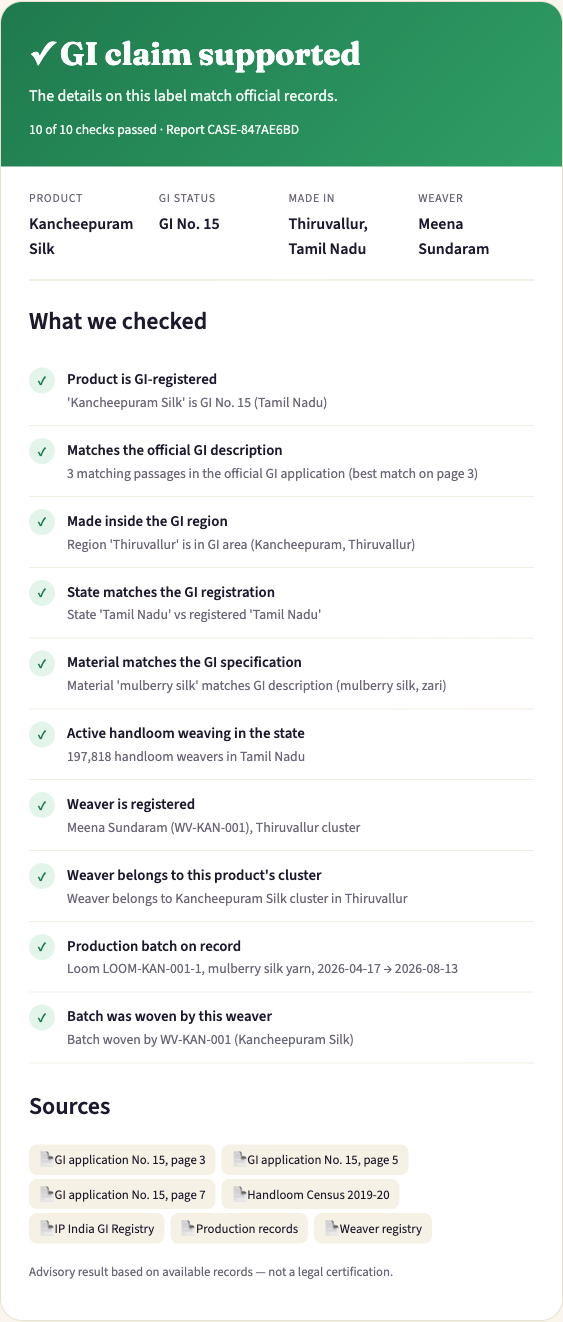
\includegraphics[width=\linewidth,height=8.5cm,keepaspectratio]{figures/ui_supported.png}\\[2pt]
{\footnotesize (a) Supported (alias resolved)}
\end{minipage}\hfill
\begin{minipage}[t]{0.48\linewidth}\centering
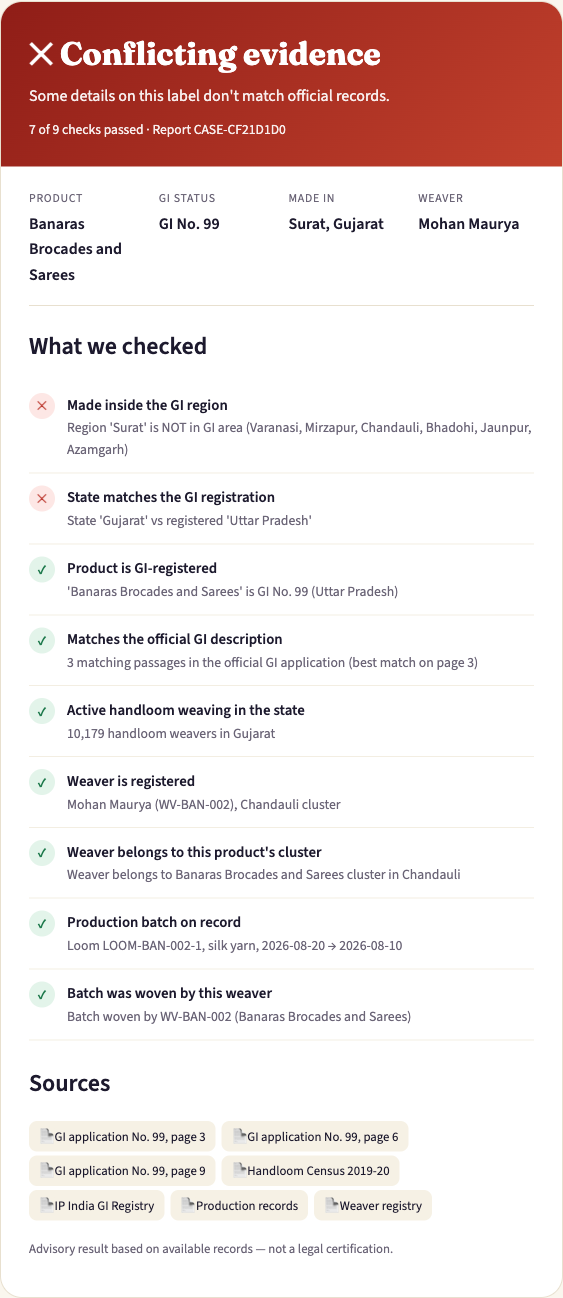
\includegraphics[width=\linewidth,height=8.5cm,keepaspectratio]{figures/ui_conflicting.png}\\[2pt]
{\footnotesize (b) Conflicting evidence (wrong region)}
\end{minipage}
\caption{Verification reports produced by the interface for two claims}
\label{fig:ui}
\end{figure}

\section{Repository Structure}

Listing~\ref{lst:repo} shows the layout of the repository and the purpose of each main file.

\begin{lstlisting}[language={},numbers=none,caption={Repository layout},label={lst:repo}]
loomtrace/
|-- README.md             # setup and run instructions
|-- requirements.txt      # streamlit, langgraph, pydantic, pandas, groq
|-- app.py                # Streamlit website (6 pages)
|-- run_tests.py          # 15 demonstration cases -> TEST_RESULTS.md
|-- loomtrace/
|   |-- agent.py          # CaseState, 6 nodes, graph, guardrail, SLM wrapper, baseline
|   |-- tools.py          # 7 tools, BM25 index, SQLite tables, review helpers
|   |-- data.py           # registry (15 GIs), census (31 rows), passages,
|   |                     #   simulated weaver and batch generator
|   |-- evaluate.py       # 45-case golden set and metrics
|   |-- experiments.py    # repeated evaluation and A/B experiment -> results/
|-- results/experiments.json  # raw numbers used in Chapters 7 and 8
|-- loomtrace.db          # SQLite: checkpoints, cases, review_queue, decisions
\end{lstlisting}

%---------------------------------------------------------------------
\chapter{Observability and Evaluation}
%---------------------------------------------------------------------

This chapter describes what is recorded for every run and reports how well the agent performs. All
numbers come from runs of the scripts \texttt{loomtrace/experiments.py} and \texttt{run\_tests.py} on
11 November 2026 on the hardware described in Section~3.5; the raw output is stored in
\texttt{results/experiments.json} and \texttt{TEST\_RESULTS.md}. All runs used the deterministic rule
mode, without a language model.

\section{Tracing and Monitoring}

Three levels of information are captured for every case.

\begin{enumerate}[itemsep=2pt]
\item \textbf{Node trace.} Each node appends an entry with its name, a summary message and a
timestamp; the planner's entry includes the plan and query, the verifier's includes every check with
its status, reason and source, and the grader's includes completeness, consistency, citation fraction
and its decision. Listings~\ref{lst:replan} and~\ref{lst:hitl} show two such traces.
\item \textbf{Tool log.} Each tool call is recorded with its iteration, input-derived source
identifier, success flag, note and elapsed time in milliseconds (Listing~\ref{lst:tools}).
\item \textbf{Checkpoints.} After every node, the complete state is serialised to JSON and stored in the
\texttt{checkpoints} table with the case identifier, step number and node name
(Listing~\ref{lst:ckpt}). The \texttt{cases}, \texttt{review\_queue} and \texttt{decisions} tables
record the outcome of each case and of each human review.
\end{enumerate}

Because all model calls were disabled, token usage and monetary cost were zero for every run and are
not reported further. Latency was measured with a high-resolution timer around each complete graph
invocation, including the SQLite writes. Over three repetitions of the 45-case set, the mean latency
of the full agent was 16.7\,ms per case (standard deviation of the three repetition means 2.9\,ms).
The slowest single case took 391.5\,ms; it was the first case of the first repetition and includes
one-time start-up work. In the second and third repetitions, no case took longer than 25\,ms. These values are four
orders of magnitude below the 15-second requirement (NFR1), as expected for a configuration without
model calls.

\section{Evaluation Dataset}

The golden set contains 45 cases: 3 products (Kancheepuram Silk, Pochampalli Ikat, and Banaras
Brocades and Sarees) $\times$ 3 verdict classes $\times$ 5 cases, the structure specified in the design
document. Each case is a label text with product, region and state, and, depending on the case,
material, weaver identifier and batch identifier. The cases are generated by the script
\texttt{evaluate.py} from the registry and the simulated producer records according to fixed rules:

\begin{itemize}[itemsep=2pt]
\item \textbf{Supported (5 per product).} A real weaver of the product and one of that weaver's
batches, the weaver's district as region, and the batch's yarn as material. Two of the five use a
market alias instead of the registered name (``Kanjivaram Silk Saree'', ``Pochampally Ikat Saree'',
``Banarasi Silk Saree'').
\item \textbf{Conflicting evidence (5 per product).} One case for each of five contradictions: a region
outside the GI area (Surat, Bhagalpur or Murshidabad); a weaver and batch from a different product's
cluster; a batch belonging to a different weaver of the same product; a product name that is not a
covered GI (``Mysore Silk Saree''); and a material inconsistent with the registration (polyester).
\item \textbf{Insufficient evidence (5 per product).} Weaver missing; batch missing; both missing; an
unknown weaver identifier (\texttt{WV-XXX-999}); and an unknown batch identifier (\texttt{B-XXX-0000}).
\end{itemize}

The label of each case is assigned by construction from these definitions, which were written by the
team before evaluation; the labels were not assigned independently by two annotators. The class
distribution is balanced, 15 cases per class. The test set was not fully separate from development:
as described in Section~7.6, one verification rule was changed after the first evaluation run revealed
three errors on this set. In addition, a separate set of 15 hand-written demonstration cases
(\texttt{run\_tests.py}) covers nine of the fifteen products, including four products that are not in
the golden set (Sambalpuri Bandha, Muga Silk, Kota Doria and Chanderi Sarees) and Kullu Shawls.

\section{Metrics and Evaluation Rubric}

Let $N = 45$ and let $y_k$ and $\hat{y}_k$ be the labelled and predicted verdicts of case $k$. The
following metrics are used.

\begin{itemize}[itemsep=2pt]
\item \textbf{Verdict accuracy} $= \frac{1}{N}\sum_k \mathbb{1}[\hat{y}_k = y_k]$.
\item \textbf{Per-class precision, recall and F1}, with $F_1 = \frac{2PR}{P+R}$, and \textbf{macro-F1}, the
unweighted mean of the three class F1-scores.
\item \textbf{Correct abstention}: the fraction of cases labelled \emph{Insufficient evidence} that are
predicted as \emph{Insufficient evidence} and therefore sent to human review.
\item \textbf{False Supported}: the number of cases predicted \emph{Supported} whose label is not
\emph{Supported}. This is the most harmful error, because it endorses an unsupported claim.
\item \textbf{Retrieval Recall@5}: the fraction of cases in which the final document search returns at
least one passage of the correct product among its top five results.
\item \textbf{Citation rate}: the fraction of decided verdicts (\emph{Supported} or \emph{Conflicting})
that list at least one source identifier.
\item \textbf{Latency and tool calls}: mean wall-clock time and mean number of tool calls per case.
\end{itemize}

The design document also proposed \emph{citation faithfulness}, the share of verdict statements backed
by the cited text, measured manually. This was not measured: the citation rate above records only that
citations are present, not that each cited passage supports the statement. No model was used as a
judge, because every output is a discrete label or check status with an exact expected value, for
which exact-match metrics are more reliable than a model judge~\cite{zheng2023judge}.

\section{Baselines}

Two comparison systems were run on the same 45 cases and the same data.

\begin{enumerate}[itemsep=2pt]
\item \textbf{Single-lookup baseline.} This follows the baseline of the design document: one document
search using the whole label as the query, followed by one decision. Because no language model was
used, the decision step is the rule ``\emph{Supported} if the top passage scores above 2, otherwise
\emph{Insufficient evidence}''. The baseline has no planning, no producer checks, no loop and no
guardrail. It is a weak baseline, and it is reported to show what retrieval alone achieves.
\item \textbf{LoomTrace without re-planning.} The full agent with the iteration limit set to one, so
that the grader can never loop back. This is the variant~A of the experiment in Chapter~8 and isolates
the contribution of the agentic loop.
\end{enumerate}

\section{Results}

Table~\ref{tab:results} summarises the results. Because the system and the baseline are deterministic,
the three repetitions produced identical verdicts, and the standard deviation of every quality metric
is zero; only latency varied between repetitions.

\begin{table}[H]
\centering
\caption{Evaluation results on the 45-case golden set (mean of 3 repetitions)}
\label{tab:results}
\small
\begin{tabularx}{\linewidth}{@{}>{\raggedright\arraybackslash}X c c c@{}}
\toprule
\textbf{Metric} & \textbf{Single lookup} & \textbf{LoomTrace, no re-plan} & \textbf{LoomTrace (full)} \\ \midrule
Verdict accuracy & 33.3\% & 80.0\% & \textbf{100.0\%} \\
Macro-F1 & 0.17 & 0.80 & \textbf{1.00} \\
F1 Supported / Conflicting / Insufficient & 0.50 / 0.00 / 0.00 & 0.75 / 0.89 / 0.77 & 1.00 / 1.00 / 1.00 \\
Correct abstention (15 cases) & 0\% & 100\% & 100\% \\
False Supported & 30 & 0 & 0 \\
Retrieval Recall@5 & -- & 1.00 & 1.00 \\
Citation rate (decided verdicts) & -- & 100\% & 100\% \\
Mean citations per case & -- & 6.40 & 6.53 \\
Mean tool calls per case (max) & 1 (1) & 6.27 (7) & 7.07 (11) \\
Cases that re-planned & -- & 0 & 9 \\
Cases escalated to review & -- & 24 & 15 \\
Mean latency per case & -- & 13.7\,ms & 16.7\,ms \\
\bottomrule
\end{tabularx}
\end{table}

As Table~\ref{tab:results} shows, the single-lookup baseline labels every case \emph{Supported}: the
label always contains the product name, so a passage about the product is always retrieved, and the
baseline has no means of detecting a contradiction or a missing identifier. It therefore endorses all
30 conflicting and insufficient claims. The full agent classifies all 45 cases correctly, sends exactly
the 15 insufficient cases to human review, and never issues a false \emph{Supported} verdict. Nine cases
used the re-planning loop: the six \emph{Supported} cases with alias names and the three
\emph{Conflicting} cases with an unregistered product name. Table~\ref{tab:confusion} gives the
confusion matrices.

\begin{table}[H]
\centering
\caption{Confusion matrices (rows: label; columns: prediction; S = Supported, C = Conflicting, I = Insufficient)}
\label{tab:confusion}
\small
\begin{tabular}{@{}l ccc c ccc c ccc@{}}
\toprule
& \multicolumn{3}{c}{\textbf{Single lookup}} && \multicolumn{3}{c}{\textbf{No re-plan}} && \multicolumn{3}{c}{\textbf{Full}} \\
\cmidrule{2-4}\cmidrule{6-8}\cmidrule{10-12}
\textbf{Label} & S & C & I && S & C & I && S & C & I \\ \midrule
Supported & 15 & 0 & 0 && 9 & 0 & 6 && 15 & 0 & 0 \\
Conflicting & 15 & 0 & 0 && 0 & 12 & 3 && 0 & 15 & 0 \\
Insufficient & 15 & 0 & 0 && 0 & 0 & 15 && 0 & 0 & 15 \\
\bottomrule
\end{tabular}
\end{table}

Figure~\ref{fig:f1} compares the per-class F1-scores of the three systems.

\begin{figure}[H]
\centering
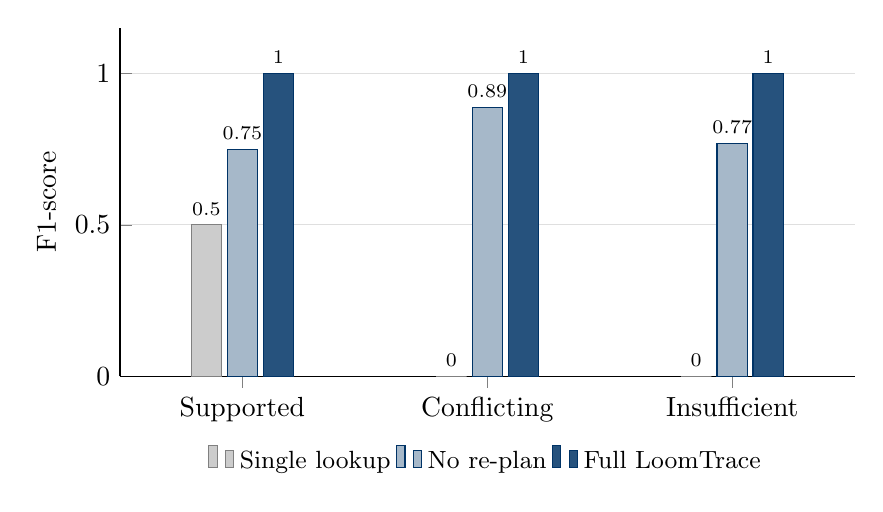
\begin{tikzpicture}
\begin{axis}[ybar,bar width=11pt,width=0.9\linewidth,height=6cm,
  ymin=0,ymax=1.15,ylabel={F1-score},
  symbolic x coords={Supported,Conflicting,Insufficient},xtick=data,
  nodes near coords,nodes near coords align={vertical},
  every node near coord/.append style={font=\scriptsize,/pgf/number format/fixed,/pgf/number format/precision=2},
  enlarge x limits=0.25,axis lines*=left,ymajorgrids,grid style={gray!25},
  legend style={at={(0.5,-0.18)},anchor=north,legend columns=3,font=\small,draw=none}]
\addplot[fill=gray!40,draw=gray] coordinates {(Supported,0.50) (Conflicting,0.00) (Insufficient,0.00)};
\addplot[fill=bmsblue!35,draw=bmsblue] coordinates {(Supported,0.75) (Conflicting,0.889) (Insufficient,0.769)};
\addplot[fill=bmsblue!85,draw=bmsblue] coordinates {(Supported,1.00) (Conflicting,1.00) (Insufficient,1.00)};
\legend{Single lookup, No re-plan, Full LoomTrace}
\end{axis}
\end{tikzpicture}
\caption{Per-class F1-score on the 45-case golden set}
\label{fig:f1}
\end{figure}

Table~\ref{tab:targets} compares the full agent with the targets set in the design document.

\begin{table}[H]
\centering
\caption{Results against the targets of the design document}
\label{tab:targets}
\small
\begin{tabularx}{\linewidth}{@{}>{\raggedright\arraybackslash}X c c >{\raggedright\arraybackslash}p{3.6cm}@{}}
\toprule
\textbf{Metric} & \textbf{Target} & \textbf{Result} & \textbf{Status} \\ \midrule
Verdict accuracy & $\geq 80\%$ & 100\% & Met \\
Retrieval Recall@5 & $\geq 0.80$ & 1.00 & Met \\
Citation faithfulness & $\geq 90\%$ & not measured & Not assessed; citation presence 100\% \\
Correct abstention & $\geq 90\%$ & 100\% & Met \\
Latency & $< 15$\,s & 16.7\,ms & Met (rule mode only) \\
\bottomrule
\end{tabularx}
\end{table}

On the 15 demonstration cases, all 15 verdicts matched the expected verdict: 7 \emph{Supported} (including
Sambalpuri Bandha, Muga Silk and Kota Doria), 5 \emph{Conflicting} (wrong region, foreign weaver, batch
of another weaver, polyester material, and a Chanderi saree claimed from Varanasi) and 3
\emph{Insufficient} (missing identifiers, unknown weaver, unknown batch). These cases are also
team-written and therefore provide functional coverage of the additional products rather than an
independent measure of accuracy.

\section{Error Analysis}

The full agent made no errors on the final golden set. This result must be read with the construction of
the test set in mind, and the analysis below therefore covers four sources of errors: errors observed
during development, errors of the ablated agent and the baseline, and errors on realistic inputs that
the golden set does not contain.

\paragraph{Errors found and corrected during development.} The first evaluation run of the full agent
reached 93.3\% accuracy (42 of 45) and 80\% correct abstention. All three errors were cases with an
unknown weaver identifier and a valid batch, labelled \emph{Insufficient} but predicted
\emph{Conflicting}, because the batch's weaver did not match the unknown identifier. The rule was
changed so that a batch--weaver mismatch is reported as \emph{unknown} when the claimed weaver itself
cannot be verified; after this change all 45 cases were correct. Because the change was made after
observing the test set, the final 100\% is partly a result of fitting to it. Separately, the
demonstration tests revealed that a claimed material of ``silk'' was rejected for Kancheepuram Silk,
whose registered material is ``mulberry silk''; the material comparison was changed to accept a match in
either direction.

\paragraph{Errors without re-planning.} All nine errors of the ablated agent fall into two categories:
six alias names that were not resolved by exact matching (\emph{Supported} predicted as
\emph{Insufficient}) and three unregistered product names that could not be classified as
\emph{Conflicting} on the first iteration. These are exactly the nine cases that the full agent resolves
by re-planning, which is analysed in Chapter~8.

\paragraph{Errors of the baseline.} All 30 errors are false \emph{Supported} verdicts, since the baseline
never checks region, state, material or producer records.

\paragraph{Errors on realistic inputs outside the test set.} To estimate behaviour beyond the constructed
cases, six further inputs that vary the spelling and form of the label were run through the full agent.
Table~\ref{tab:probes} shows the results. Four of the six produced a wrong \emph{Conflicting} verdict.

\begin{table}[H]
\centering
\caption{Behaviour on six realistic inputs not in the golden set}
\label{tab:probes}
\small
\begin{tabularx}{\linewidth}{@{}>{\raggedright\arraybackslash}p{4.4cm} >{\raggedright\arraybackslash}p{2.3cm} >{\raggedright\arraybackslash}X@{}}
\toprule
\textbf{Input variation} & \textbf{Verdict} & \textbf{Cause} \\ \midrule
Alias not in list (``Conjeevaram Silk Saree'') & Conflicting (wrong) & Product unresolved after re-plan, so the product check fails \\
District spelling (``Kanchipuram'') & Conflicting (wrong) & Region compared by substring; spelling variant not matched \\
State abbreviation (``TS'') & Conflicting (wrong) & State compared by exact name; census lookup also fails \\
Former state name (``Andhra Pradesh'' for Pochampalli) & Conflicting (wrong) & Registry stores current state (Telangana) only \\
Lower-case identifiers & Supported (correct) & Identifiers are upper-cased before lookup \\
Free-text sentence with alias and identifiers & Supported (correct) & Parser finds product alias and identifier patterns \\
\bottomrule
\end{tabularx}
\end{table}

These four failures share one cause: the region, state and product comparisons are exact or substring
matches against a single canonical spelling. They would be fixed by (i) fuzzy matching of district and
product names against the registry, with a similarity threshold below which the check is
\emph{unknown} rather than \emph{fail}; (ii) a table of state abbreviations and former state names; and
(iii) treating a product that cannot be resolved as ``not covered'' inside the agent, as the interface
already does before the agent runs. The more general lesson is that a contradiction should only be
reported when the mismatch is certain, and that uncertain mismatches should be routed to human review.

%---------------------------------------------------------------------
\chapter{Experimentation}
%---------------------------------------------------------------------

This chapter reports one controlled A/B experiment. The factor varied is the re-planning loop, which
is the main agentic element of LoomTrace: in variant~A the grader may never send control back to the
planner, and in variant~B, the default configuration, it may do so up to two times. The experiment
answers whether this loop is worth its cost.

\section{Hypothesis}

Allowing the agent to re-plan and retrieve again when the first registry lookup or document search is
inconclusive (variant~B) will increase verdict accuracy compared with a single planning pass
(variant~A), without increasing false \emph{Supported} verdicts, at a latency cost of less than one
second per case.

The hypothesis is falsifiable in three ways: accuracy could fail to rise, the loop could introduce
false \emph{Supported} verdicts by resolving names too permissively, or the extra iteration could cost
more than one second.

\section{Experimental Setup}

\paragraph{Variants.} Variant~A sets the maximum number of planning iterations to one. Variant~B sets it
to three, the value used in all other chapters. In both variants, the first iteration is identical: an
exact registry match and an unfiltered document search. Only variant~B can perform the second
iteration, which resolves aliases and filters the search to the resolved product.

\paragraph{Fixed factors.} The code, the graph, the tools, the reference data, the BM25 parameters,
the grading formula, the guardrail thresholds and the 45-case golden set were identical for both
variants. No language model was used in either variant.

\paragraph{Procedure.} The script \texttt{loomtrace/experiments.py} ran both variants on all 45 cases,
alternating A and B within each of three repetitions, so that any warm-up effect affects both variants.
For each case it recorded the verdict, the number of iterations, the number of tool calls, the number
of node executions and the wall-clock time.

\paragraph{Metrics.} Verdict accuracy, macro-F1, false \emph{Supported} verdicts and correct abstention,
as defined in Section~7.3; mean tool calls and node executions per case; and mean latency per case,
reported as the mean and standard deviation of the three repetition means.

\section{Results}

Table~\ref{tab:ab} gives the results, and Figure~\ref{fig:ab} shows accuracy and mean tool calls for
the two variants.

\begin{table}[H]
\centering
\caption{A/B experiment: single planning pass (A) versus re-planning loop (B), 45 cases, 3 repetitions}
\label{tab:ab}
\small
\begin{tabularx}{\linewidth}{@{}>{\raggedright\arraybackslash}X c c c@{}}
\toprule
\textbf{Metric} & \textbf{Variant A} & \textbf{Variant B} & \textbf{Difference (B $-$ A)} \\ \midrule
Verdict accuracy (mean $\pm$ s.d.) & 80.0\% $\pm$ 0.0 & 100.0\% $\pm$ 0.0 & +20.0 points \\
Macro-F1 & 0.80 & 1.00 & +0.20 \\
Correct abstention & 100\% & 100\% & 0 \\
False Supported & 0 & 0 & 0 \\
Cases escalated to review & 24 & 15 & $-9$ \\
Mean tool calls per case & 6.27 & 7.07 & +0.80 \\
Maximum tool calls per case & 7 & 11 & +4 \\
Mean node executions per case & 6.00 & 6.80 & +0.80 \\
Mean latency per case (mean $\pm$ s.d.) & 13.7 $\pm$ 1.7\,ms & 16.7 $\pm$ 2.9\,ms & +3.1\,ms \\
\bottomrule
\end{tabularx}
\end{table}

\begin{figure}[H]
\centering
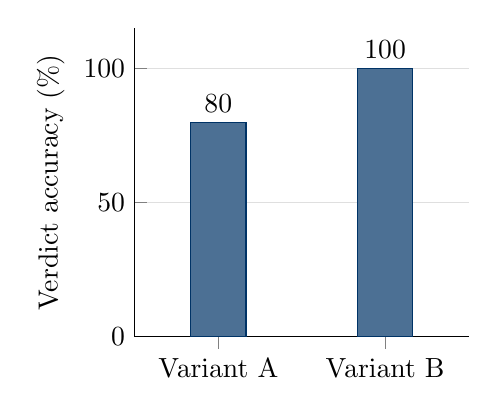
\begin{tikzpicture}
\begin{axis}[ybar,bar width=20pt,width=0.48\linewidth,height=5.5cm,
  ymin=0,ymax=115,ylabel={Verdict accuracy (\%)},
  symbolic x coords={Variant A,Variant B},xtick=data,
  nodes near coords,nodes near coords align={vertical},
  enlarge x limits=0.5,axis lines*=left,ymajorgrids,grid style={gray!25}]
\addplot[fill=bmsblue!70,draw=bmsblue] coordinates {(Variant A,80.0) (Variant B,100.0)};
\end{axis}
\end{tikzpicture}\hfill
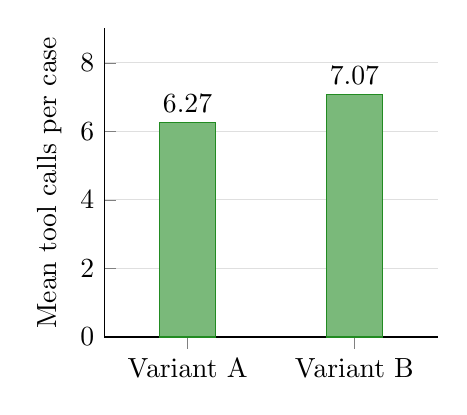
\begin{tikzpicture}
\begin{axis}[ybar,bar width=20pt,width=0.48\linewidth,height=5.5cm,
  ymin=0,ymax=9,ylabel={Mean tool calls per case},
  symbolic x coords={Variant A,Variant B},xtick=data,
  nodes near coords,nodes near coords align={vertical},
  every node near coord/.append style={/pgf/number format/fixed,/pgf/number format/precision=2},
  enlarge x limits=0.5,axis lines*=left,ymajorgrids,grid style={gray!25}]
\addplot[fill=ForestGreen!60,draw=ForestGreen] coordinates {(Variant A,6.27) (Variant B,7.07)};
\end{axis}
\end{tikzpicture}
\caption{Verdict accuracy (left) and mean tool calls per case (right) for the two variants}
\label{fig:ab}
\end{figure}

The accuracy of both variants was identical in all three repetitions, because the system is
deterministic; the variation between repetitions is confined to latency. Per-repetition mean latencies
were 11.3, 14.4 and 15.4\,ms for variant~A and 20.7, 13.8 and 15.8\,ms for variant~B. The first
repetition of variant~B includes one case of 391.5\,ms caused by start-up work, which raises that
repetition's mean; the difference in mean latency between the variants is therefore of the same order
as the variation between repetitions.

All nine cases on which the variants differ are cases in which the first iteration could not resolve
the product: in variant~A they end as \emph{Insufficient evidence}, six of which should have been
\emph{Supported} and three \emph{Conflicting}. Variant~B re-plans on exactly these nine cases and on no
others; each re-planned case executes ten nodes and eleven tool calls instead of six nodes and five to
seven tool calls.

\section{Discussion and Decision}

The hypothesis was supported on all three counts. The re-planning loop increased verdict accuracy by
20 percentage points, from 80.0\% to 100.0\%, and macro-F1 from 0.80 to 1.00. It introduced no false
\emph{Supported} verdicts, because the second iteration only resolves names that match a registered
alias and still requires every check to pass. Its cost was 0.8 additional tool calls per case on
average and an increase in mean latency of about 3\,ms, far below the one-second bound and comparable
to the run-to-run variation.

The experiment also shows where the benefit comes from. Variant~A is not unsafe: it never endorses a
false claim and it abstains on all unclear cases. Its weakness is that it abstains too often, sending
24 cases to human review instead of the 15 that genuinely require it. The loop therefore reduces the
workload of human reviewers by nine cases out of 45 (20\%) without lowering safety. In a deployment
where reviewers are the scarce resource, this is the most important effect.

Two cautions apply. First, the result was obtained on a test set in which six of 45 cases deliberately
use aliases; the size of the benefit depends on how often real labels use non-registered names. Second,
Chapter~7 showed that names outside the alias list are not resolved even with re-planning, so the loop
helps only as far as the alias table and matching rules allow. \textbf{Decision:} variant~B, with a
maximum of three planning iterations, was adopted as the default configuration, because it improves
accuracy and reduces reviewer workload at negligible cost and with no loss of safety.

%---------------------------------------------------------------------
\chapter{Limitations, Ethics and Safety}
%---------------------------------------------------------------------

This chapter states the limitations of the data, the method and the evaluation, lists the ways in
which the agent can fail together with the guardrail that addresses each, and discusses the ethical
considerations of a system whose output affects producers and buyers.

\section{Limitations}

\paragraph{Data.} The producer-level evidence, the weaver registry and the batch records, is simulated.
Real individual records are not published, so the weaver and batch checks demonstrate the mechanism
but say nothing about the availability or quality of real records. The GI description passages for the
three original products were written by the team as summaries and their page references are
indicative; they were not extracted from the scanned GI application documents. For the twelve products
taken from the government GI catalogue, the descriptions are short and the catalogue does not give GI
application numbers. The registry stores one current state per product, so historical state names, such
as Andhra Pradesh for products now in Telangana, are not recognised.

\paragraph{Method.} All factual checks are deterministic string comparisons. As shown in
Table~\ref{tab:probes}, spelling variants of districts, state abbreviations and aliases that are not in
the alias table lead to wrong \emph{Conflicting} verdicts. Retrieval uses BM25 over 21 short passages,
which is adequate for this corpus but would not scale to the full text of GI applications without dense
retrieval and chunking. The language-model path for extraction and explanation is implemented but was
not evaluated, and the OCR path for label images was not installed or tested. The durable-workflow
support stores every state but does not resume interrupted runs automatically.

\paragraph{Evaluation.} The 45-case golden set and the 15 demonstration cases were constructed by the
team from the same rules and records that the agent uses, the labels were assigned by construction
rather than by independent annotators, and one rule was changed after the first evaluation run. The
100\% accuracy therefore shows that the agent behaves as designed on controlled cases; it is not an
estimate of accuracy on real marketplace listings. Citation faithfulness was not measured. The golden
set covers three of the fifteen products. The single-lookup baseline is weak by design.

\section{Failure Modes and Guardrails}

Table~\ref{tab:failures} pairs each identified failure mode with its mitigation.

\begin{table}[H]
\centering
\caption{Failure modes and mitigations}
\label{tab:failures}
\small
\begin{tabularx}{\linewidth}{@{}>{\raggedright\arraybackslash}X >{\raggedright\arraybackslash}X@{}}
\toprule
\textbf{Failure mode} & \textbf{Mitigation} \\ \midrule
Verdict issued without evidence & Citation gate: a decided verdict needs at least one source ID and a grade $\geq 0.6$, otherwise it is downgraded to \emph{Insufficient} and escalated \\
Weak or off-product retrieval & Grader detects unresolved product or weak search; planner re-queries with canonical name and product filter; maximum three iterations \\
Unbounded looping or tool calls & Iteration limit of 3 and a graph recursion limit of 40; observed maximum 2 iterations and 11 tool calls \\
Missing weaver or batch details & Checks marked \emph{unknown}, never \emph{pass}; case escalated to review with the missing items listed \\
Typing error in an identifier & Unknown identifier gives \emph{unknown}, not \emph{fail}; batch mismatch is not asserted against an unverified weaver \\
Spelling variants causing false conflicts (observed, Table~\ref{tab:probes}) & Not yet mitigated in the agent; planned fuzzy matching with an \emph{unknown} band, and abbreviation and former-name tables (Section~10.2) \\
Product outside the covered GIs & Interface reports ``not covered'' before the agent runs and offers referral to a reviewer \\
Model returns malformed or invented fields & JSON mode, Pydantic validation and deterministic fall-back parser; the model never performs factual checks \\
Instructions embedded in label text (prompt injection) & Label text is only parsed into fields; tools are fixed by the graph, not chosen by the model; the explanation prompt receives only check statuses, source IDs and tool notes \\
Reviewer error or bias & Reviewer must record a note; the decision is stored with the automated verdict, so both remain auditable \\
\bottomrule
\end{tabularx}
\end{table}

\section{Ethical and Responsible-Use Considerations}

\paragraph{Who could be harmed.} A wrong \emph{Conflicting} verdict on a genuine product could damage the
reputation and sales of a weaver who is legitimately entitled to the GI, and Chapter~7 showed that
spelling variants can produce exactly this error. A wrong \emph{Supported} verdict would mislead a buyer
and undermine the value of the GI for all producers in the region. The design therefore treats a false
\emph{Supported} verdict as the most serious error, and none occurred in the evaluation; the observed
false \emph{Conflicting} verdicts on realistic spelling variants are the most important weakness to
correct before any real use.

\paragraph{Advisory status.} Every verdict is labelled in the interface as ``advisory result based on
available records --- not a legal certification''. Authority over GI registration and authorised use
rests with the GI Registry under the GI Act~\cite{giact1999}, and the system does not claim to replace
it. Every verdict shows the checks performed and the sources used, so that a user can see why it was
reached, and any user can send a decided case to a human reviewer.

\paragraph{Human oversight.} Cases that the agent cannot decide are never resolved automatically. They
are routed to a reviewer, whose decision and note are stored separately from the automated verdict and
shown to the requester. This keeps a person accountable for every decision that is not fully supported
by evidence.

\paragraph{Privacy.} Weaver records can contain personal information. In this project, all weaver
records are simulated, and the names are randomly combined from lists of common first names and
surnames; they do not refer to real people. A real deployment would require consent from weavers and
cooperatives, access control on the weaver registry and the review dashboard, and a retention policy
for case data, which are not implemented here; the current Admin page has no authentication.

\paragraph{Fairness.} Coverage is uneven: fifteen GIs are supported, the alias table reflects the names
known to the team, and products from regions with less documentation are more likely to be marked
\emph{Insufficient} or ``not covered''. This should be reduced by extending coverage with producer
associations rather than by relaxing the checks.

%---------------------------------------------------------------------
\chapter{Conclusion and Future Work}
%---------------------------------------------------------------------

\section{Conclusion}

This report addressed the problem of checking whether a GI-tag claim on an Indian handloom product is
supported by official evidence, a task for which the necessary information is spread across the GI
registry, GI descriptions, the national handloom census and producer records. It presented LoomTrace,
an agent implemented as a six-node LangGraph state graph with seven typed tools, retrieval over official
GI text, a bounded re-planning loop, an evidence grader, a citation and confidence guardrail, and a
human review workflow, covering fifteen registered handloom GIs.

The objectives stated in Section~1.4 were addressed as follows.

\begin{enumerate}[itemsep=2pt]
\item \textbf{Agent design.} Met. The state-graph agent returns one of three verdicts with the result
and source of every check (Chapter~4).
\item \textbf{Tools, retrieval and bounded re-planning.} Met. Seven typed tools and a BM25 index over
21 passages were implemented; the loop is limited to three iterations and in practice used at most two
(Chapter~6).
\item \textbf{Guardrail and human review.} Met. All 15 unclear cases in the test set were escalated, and
reviewer decisions with notes are recorded and shown to the requester (Chapters~5 and~7).
\item \textbf{Tracing and checkpoints.} Met. Every node writes a trace entry and a checkpoint; LangSmith,
proposed in the design document, was replaced by this local store (Chapter~5).
\item \textbf{Evaluation against a baseline.} Met for accuracy and abstention. On the 45-case golden set
the agent reached 100\% accuracy and 100\% correct abstention against targets of 80\% and 90\%, while a
single-lookup baseline reached 33.3\% and 0\%. Citation faithfulness was not measured, and the result
holds for team-constructed cases only; on six realistic spelling variants the agent produced four wrong
\emph{Conflicting} verdicts (Chapter~7).
\item \textbf{A/B experiment.} Met. Disabling re-planning reduced accuracy from 100\% to 80\% and
increased escalations from 15 to 24, while the loop cost 0.8 tool calls and about 3\,ms per case;
re-planning was adopted as the default (Chapter~8).
\end{enumerate}

The main conclusion is that, for this verification task, the agentic elements contribute through
control rather than through generation: re-planning recovers cases that a single pass would wrongly
leave undecided, and the guardrail ensures that undecidable cases reach a person instead of receiving
a guessed verdict.

\section{Future Work}

The following extensions follow directly from the limitations in Chapter~9.

\begin{enumerate}[itemsep=2pt]
\item \textbf{Robust name matching.} Add fuzzy matching of product, district and state names with a
similarity band in which checks are marked \emph{unknown} rather than \emph{fail}, together with tables
of state abbreviations and former state names, so that the four failures in Table~\ref{tab:probes}
become correct or escalated verdicts.
\item \textbf{Official GI application text.} Download and OCR the statements of case of the covered GIs
from the IP India registry, index them with chunking and dense retrieval, and record the GI application
numbers of all fifteen products, replacing the team-written summaries and indicative page numbers.
\item \textbf{Real producer data.} Replace the simulated weaver and batch records with records from a
partner weavers' cooperative, with consent and access control, and evaluate on real labels.
\item \textbf{Independent evaluation.} Build a test set from real marketplace listings labelled by two
independent annotators, measure inter-annotator agreement and citation faithfulness, and evaluate the
language-model extraction path on it.
\item \textbf{Automatic resumption.} Use the stored checkpoints to resume interrupted runs and to pause
the graph at the review step, so that a reviewer's decision continues the same run.
\end{enumerate}


%=====================================================================
%  REFERENCES
%=====================================================================
\begin{thebibliography}{99}
\addcontentsline{toc}{chapter}{References}

\bibitem{yao2023react} S.~Yao, J.~Zhao, D.~Yu, N.~Du, I.~Shafran, K.~Narasimhan, and Y.~Cao,
``ReAct: Synergizing reasoning and acting in language models,'' in \emph{Proc. Int. Conf. Learning
Representations (ICLR)}, 2023.

\bibitem{lewis2020rag} P.~Lewis \emph{et al.}, ``Retrieval-augmented generation for knowledge-intensive
NLP tasks,'' in \emph{Advances in Neural Information Processing Systems (NeurIPS)}, vol.~33, 2020.

\bibitem{schick2023toolformer} T.~Schick \emph{et al.}, ``Toolformer: Language models can teach
themselves to use tools,'' in \emph{Advances in Neural Information Processing Systems (NeurIPS)}, 2023.

\bibitem{shinn2023reflexion} N.~Shinn, F.~Cassano, A.~Gopinath, K.~Narasimhan, and S.~Yao,
``Reflexion: Language agents with verbal reinforcement learning,'' in \emph{Advances in Neural
Information Processing Systems (NeurIPS)}, 2023.

\bibitem{asai2024selfrag} A.~Asai, Z.~Wu, Y.~Wang, A.~Sil, and H.~Hajishirzi, ``Self-RAG: Learning to
retrieve, generate, and critique through self-reflection,'' in \emph{Proc. Int. Conf. Learning
Representations (ICLR)}, 2024.

\bibitem{yan2024crag} S.-Q.~Yan, J.-C.~Gu, Y.~Zhu, and Z.-H.~Ling, ``Corrective retrieval augmented
generation,'' \emph{arXiv preprint arXiv:2401.15884}, 2024.

\bibitem{wu2023autogen} Q.~Wu \emph{et al.}, ``AutoGen: Enabling next-gen LLM applications via
multi-agent conversation,'' \emph{arXiv preprint arXiv:2308.08155}, 2023.

\bibitem{wang2024survey} L.~Wang \emph{et al.}, ``A survey on large language model based autonomous
agents,'' \emph{Frontiers of Computer Science}, vol.~18, no.~6, 2024.

\bibitem{zheng2023judge} L.~Zheng \emph{et al.}, ``Judging LLM-as-a-judge with MT-Bench and Chatbot
Arena,'' in \emph{Advances in Neural Information Processing Systems (NeurIPS), Datasets and Benchmarks
Track}, 2023.

\bibitem{wang2023plansolve} L.~Wang \emph{et al.}, ``Plan-and-solve prompting: Improving zero-shot
chain-of-thought reasoning by large language models,'' in \emph{Proc. 61st Annu. Meeting of the
Association for Computational Linguistics (ACL)}, 2023.

\bibitem{robertson2009bm25} S.~Robertson and H.~Zaragoza, ``The probabilistic relevance framework:
BM25 and beyond,'' \emph{Foundations and Trends in Information Retrieval}, vol.~3, no.~4,
pp.~333--389, 2009.

\bibitem{ji2023hallucination} Z.~Ji \emph{et al.}, ``Survey of hallucination in natural language
generation,'' \emph{ACM Computing Surveys}, vol.~55, no.~12, 2023.

\bibitem{liu2024lost} N.~F.~Liu \emph{et al.}, ``Lost in the middle: How language models use long
contexts,'' \emph{Transactions of the Association for Computational Linguistics}, vol.~12, 2024.

\bibitem{gao2023ragsurvey} Y.~Gao \emph{et al.}, ``Retrieval-augmented generation for large language
models: A survey,'' \emph{arXiv preprint arXiv:2312.10997}, 2023.

\bibitem{llama3} A.~Grattafiori \emph{et al.}, ``The Llama 3 herd of models,'' \emph{arXiv preprint
arXiv:2407.21783}, 2024.

\bibitem{giact1999} Government of India, ``The Geographical Indications of Goods (Registration and
Protection) Act, 1999,'' Act No.~48 of 1999, Ministry of Law, Justice and Company Affairs, 1999.

\bibitem{trips} World Trade Organization, ``Agreement on Trade-Related Aspects of Intellectual
Property Rights,'' Annex 1C of the Marrakesh Agreement, Part~II, Section~3 (Articles 22--24), 1994.

\bibitem{ipindia} Office of the Controller General of Patents, Designs and Trade Marks,
``Geographical Indications Registry,'' Intellectual Property India. [Online]. Available:
\url{https://ipindia.gov.in}. Accessed: Nov.~2026.

\bibitem{pibcensus} Ministry of Textiles, Government of India, ``State/UT-wise number of handloom
weavers and allied workers as per 4th All India Handloom Census 2019--20,'' Annexure to Press
Information Bureau release ID 2202869, Dec.~2025. [Online]. Available:
\url{https://static.pib.gov.in/WriteReadData/specificdocs/documents/2025/dec/doc20251212729201.pdf}.
Accessed: Nov.~2026.

\bibitem{pibgi} Tribal Co-operative Marketing Development Federation of India (TRIFED), Ministry of
Tribal Affairs, ``Geographical Indications of India,'' Press Information Bureau document, Nov.~2021.
[Online]. Available:
\url{https://static.pib.gov.in/WriteReadData/specificdocs/documents/2021/nov/doc2021112441.pdf}.
Accessed: Nov.~2026.

\bibitem{handloommark} Office of the Development Commissioner (Handlooms), Ministry of Textiles,
``Handloom Mark and India Handloom Brand schemes.'' [Online]. Available:
\url{https://handlooms.nic.in}. Accessed: Nov.~2026.

\bibitem{langgraph} LangChain Inc., ``LangGraph documentation,'' 2025. [Online]. Available:
\url{https://langchain-ai.github.io/langgraph/}. Accessed: Nov.~2026.

\bibitem{pydantic} S.~Colvin \emph{et al.}, ``Pydantic: Data validation using Python type hints,''
2025. [Online]. Available: \url{https://docs.pydantic.dev}. Accessed: Nov.~2026.

\bibitem{streamlit} Snowflake Inc., ``Streamlit documentation,'' 2025. [Online]. Available:
\url{https://docs.streamlit.io}. Accessed: Nov.~2026.

\bibitem{groq} Groq Inc., ``GroqCloud API documentation: supported models,'' 2025. [Online].
Available: \url{https://console.groq.com/docs/models}. Accessed: Nov.~2026.

\bibitem{easyocr} JaidedAI, ``EasyOCR: Ready-to-use OCR with 80+ supported languages,'' GitHub
repository. [Online]. Available: \url{https://github.com/JaidedAI/EasyOCR}. Accessed: Nov.~2026.

\bibitem{sqlite} D.~R.~Hipp, ``SQLite,'' 2025. [Online]. Available: \url{https://www.sqlite.org}.
Accessed: Nov.~2026.

\end{thebibliography}


%=====================================================================
%  APPENDICES
%=====================================================================
\appendix
\chapter{Team Contribution}
\label{app:contrib}

Table~\ref{tab:contrib} lists the components owned by each member, following the roles assigned in the
project's design document. All members took part in the reviews and are able to explain the complete
system.

\begin{table}[H]
\centering
\caption{Contribution of team members}
\label{tab:contrib}
\small
\begin{tabularx}{\linewidth}{@{}l l X c@{}}
\toprule
\textbf{USN} & \textbf{Name} & \textbf{Components owned} & \textbf{Share} \\ \midrule
\USNa & \NameA\ (Lead) & Project coordination, problem charter, design document, documentation and report & 25\% \\
\USNb & \NameB & Agent and RAG implementation: graph, CaseState, planner, grader, re-planning loop, guardrail, retrieval index, prompts & 25\% \\
\USNc & \NameC & Data collection (GI registry, PIB catalogue, census), simulated records, tools, web interface & 25\% \\
\USNd & \NameD & Golden test set, metrics, baseline, A/B experiment, demonstration tests, error analysis & 25\% \\
\bottomrule
\end{tabularx}
\end{table}

\chapter{Setup and Run Instructions}
\label{app:run}

The source code, the evaluation results and the source of this report are available at
\url{https://github.com/hrterrain/loomtrace-agent}. The system runs on any computer with Python~3.11 or later; no graphics processor or internet
connection is needed in rule mode. The commands below create the environment, start the interface and
reproduce every number in Chapters~7 and~8.

\begin{lstlisting}[language={},numbers=none]
git clone https://github.com/hrterrain/loomtrace-agent.git
cd loomtrace-agent
python3 -m venv .venv && source .venv/bin/activate
pip install -r requirements.txt          # streamlit, langgraph, pydantic, pandas, groq

# optional: enable Llama 3.1 8B on Groq for extraction and explanations
export GROQ_API_KEY=<your key>          # never commit the key

# optional: label images
pip install easyocr

streamlit run app.py                     # web interface on http://localhost:8501
python -m loomtrace.experiments          # Tables 7.1-7.3 and 8.1 -> results/experiments.json
python -m loomtrace.evaluate             # single 45-case evaluation
python run_tests.py                      # 15 demonstration cases -> TEST_RESULTS.md
\end{lstlisting}

Versions used for the reported runs: Python 3.13.7, LangGraph 1.2.20, langchain-core 1.7.7,
Pydantic 2.14.3, Streamlit 1.67.0, pandas 3.1.1, groq 1.7.0, on macOS 15.6 (Apple M2, 8\,GB). The SQLite
database \texttt{loomtrace.db} is created automatically on first run.

\chapter{Sample Traces and Screenshots}

This appendix gives three complete runs: a successful run, a run that required a correction through
re-planning, and an abstention. All were produced by the system on 11 November 2026.

\section{Successful Run with Correction: Kanjivaram Silk Saree}

The node trace of this run is Listing~\ref{lst:replan}, its tool log is Listing~\ref{lst:tools}, and
its checkpoints are Listing~\ref{lst:ckpt}. The first iteration could not resolve the alias
``Kanjivaram'' (grade 0.65); the second resolved it to Kancheepuram Silk, all ten checks passed (grade
1.0), and the verdict \emph{Supported} was issued with seven citations: \texttt{GI15-p3},
\texttt{GI15-p5}, \texttt{GI15-p7}, \texttt{HLCENSUS-2019-20\#Tamil\_Nadu},
\texttt{IPINDIA-GI-REG\#15}, \texttt{SIM-PROV\#B-KAN-0010} and \texttt{SIM-WEAVER\#WV-KAN-001}. The
report shown to the requester is Fig.~\ref{fig:ui}(a).

\section{Contradiction: Banarasi Saree Claimed from Surat}

Listing~\ref{lst:conflict} shows a claim for a Banarasi silk saree said to be made in Surat, Gujarat,
with a valid Banaras weaver and batch. The alias required one re-plan; the verifier then found two
failed checks, and the grader's consistency score of 0 led to \emph{Conflicting evidence}. The report is
Fig.~\ref{fig:ui}(b).

\begin{lstlisting}[language={},caption={Trace of a conflicting claim (case REPORT-TRACE-3)},label={lst:conflict}]
{"node": "Extract",   "msg": "parsed label text: product=Banarasi Silk Saree,
   region=Surat, state=Gujarat, weaver_id=WV-BAN-002, batch_id=B-BAN-0020"}
{"node": "Planner",   "msg": "Initial plan: exact registry match, unfiltered
   document search"}
{"node": "Retriever", "msg": "gi_registry_lookup X . gi_doc_search OK .
   census_lookup OK . weaver_lookup OK . provenance_lookup OK"}
{"node": "Verifier",  "msg": "5 pass . 0 fail . 4 unknown"}
{"node": "Grader",    "msg": "grade=0.69 (completeness 0.56, consistency 1.0)
   -> re-plan"}
{"node": "Planner",   "msg": "Re-plan #1: resolve aliases -> 'Banaras Brocades
   and Sarees', sharper query filtered by product"}
{"node": "Retriever", "msg": "gi_registry_lookup OK . gi_doc_search OK .
   census_lookup OK . weaver_lookup OK . provenance_lookup OK"}
{"node": "Verifier",  "msg": "7 pass . 2 fail . 0 unknown"}
{"node": "Grader",    "msg": "grade=1.0 (completeness 1.0, consistency 0.0)
   -> finish"}
{"node": "Guardrail", "msg": "Conflicting evidence"}
rationale: "Conflict found: Region 'Surat' is NOT in GI area (Varanasi,
  Mirzapur, Chandauli, Bhadohi, Jaunpur, Azamgarh); State 'Gujarat' vs
  registered 'Uttar Pradesh'."
\end{lstlisting}

\section{Abstention: Banaras Saree without Producer Details}

The trace of this run is Listing~\ref{lst:hitl}. Figure~\ref{fig:insuff} shows the report presented to
the requester, which states that the case has been sent to an expert reviewer and lists the four
producer checks that could not be made. The reviewer's dashboard and the requester's tracking view for
such a case are Figs.~\ref{fig:admin} and~\ref{fig:track}.

\begin{figure}[H]
\centering
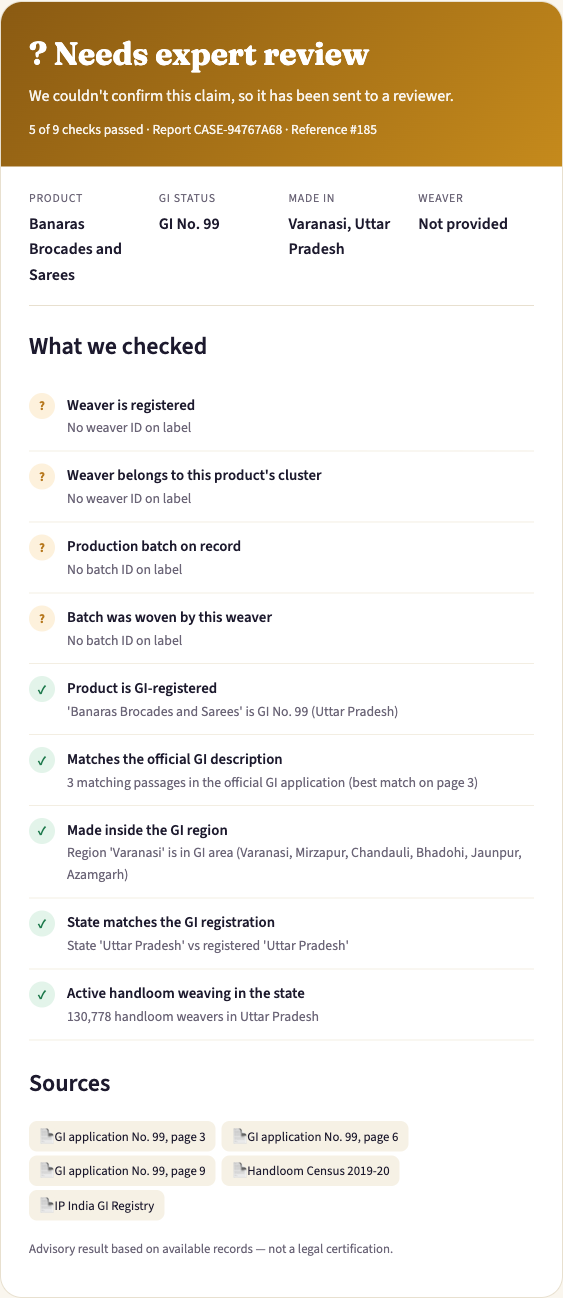
\includegraphics[width=0.5\linewidth]{figures/ui_insufficient.png}
\caption{Report for a claim without weaver or batch details, escalated to human review}
\label{fig:insuff}
\end{figure}

\chapter{Prompts}
\label{app:prompts}

LoomTrace uses a language model only in the optional model mode, for two tasks. Both prompts are sent
as the system message to \texttt{llama-3.1-8b-instant} on Groq with temperature 0 and
\texttt{response\_format=\{"type": "json\_object"\}}. As stated in Section~6.5, these prompts were not
used in the reported evaluation. No model is used as a judge, so there is no judge rubric.

\begin{lstlisting}[language={},caption={System prompt for field extraction; the user message is the label text}]
Extract handloom label fields. Return JSON with keys: product, region (district),
state, weaver_id, batch_id, material, gi_claim (bool). Use null if absent.
Copy IDs exactly.
\end{lstlisting}

\begin{lstlisting}[language={},caption={System prompt for the verdict explanation; the user message is a JSON object with the verdict, the status of each check and up to twelve source IDs with notes}]
You explain a GI verification verdict in 2-3 sentences. Only use the given checks
and cite sources in [brackets]. Return JSON {"rationale": str}.
\end{lstlisting}

The extraction prompt asks for a fixed key set so that the output can be validated by the
\texttt{LabelFields} model, requires \texttt{null} for absent fields so that missing information is not
invented, and requires identifiers to be copied exactly because they are used as database keys. The
explanation prompt limits the model to the checks already computed, so that the explanation cannot
introduce facts that were not verified. If either call fails or returns invalid JSON, the deterministic
parser or the template explanation is used instead.


\end{document}
